\documentclass[11pt,letterpaper]{article}

\usepackage[margin=1in]{geometry}
\usepackage{setspace}
\onehalfspacing

\usepackage{microtype}
\usepackage{titlesec}
\usepackage{enumitem}
\usepackage{booktabs}
\usepackage{longtable}
\usepackage{multirow}
\usepackage{array}
\usepackage{tabularx}
\usepackage{xcolor}
\usepackage{colortbl}

\usepackage{tikz}
\usetikzlibrary{shapes.geometric, arrows.meta, positioning, fit, backgrounds, calc, decorations.pathreplacing, patterns, shadows, chains}
\usepackage{pgfplots}
\pgfplotsset{compat=1.18}

\usepackage{listings}
\lstset{
    basicstyle=\ttfamily\small,
    breaklines=true,
    frame=single,
    backgroundcolor=\color{gray!10},
    keywordstyle=\color{blue},
    commentstyle=\color{green!50!black},
    stringstyle=\color{red!70!black},
    numbers=left,
    numberstyle=\tiny\color{gray},
    numbersep=5pt,
}

\usepackage{amsmath,amssymb,amsthm}

\usepackage[hyphens]{url}
\usepackage[colorlinks=true,linkcolor=blue,citecolor=blue,urlcolor=blue]{hyperref}
\usepackage{cleveref}

\usepackage[numbers,sort&compress]{natbib}

\definecolor{ucxblue}{RGB}{0,102,204}
\definecolor{ncclgreen}{RGB}{118,185,0}
\definecolor{cudaorange}{RGB}{255,153,0}
\definecolor{rdmared}{RGB}{204,0,0}
\definecolor{problemred}{RGB}{220,53,69}
\definecolor{solutiongreen}{RGB}{40,167,69}
\definecolor{layergray}{RGB}{240,240,240}
\definecolor{neumannpurple}{RGB}{102,51,153}
\definecolor{v100blue}{RGB}{30,90,180}
\definecolor{tower1color}{RGB}{50,130,60}
\definecolor{tower2color}{RGB}{130,50,50}
\definecolor{wfapurple}{RGB}{102,51,153}

\theoremstyle{definition}
\newtheorem{challenge}{Challenge}
\newtheorem{designchoice}{Design Choice}
\newtheorem{solution}{Proposed Solution}

\title{
    \vspace{-1cm}
    \textbf{Adaptive RDMA Optimization for Distributed LLM Workloads} \\[0.5em]
    \large A Consolidated Technical Report
}

\author{
    Nathan Gopee \\
    \textit{MS Computer Science Candidate} \\
    SUNY New Paltz \\
    \texttt{gopeen1@newpaltz.edu} \\[1em]
    \small Advisors: Dr.\ Wafi Danesh \& Dr.\ Ashley Suchy
}

\date{February 2026}

\begin{document}

\maketitle

\begin{abstract}
\noindent
\textbf{Project Purpose.}
When you run a large language model across multiple GPUs, those GPUs spend 30--60\% of their cycles waiting for data to arrive over the network. Existing communication libraries (NCCL, Gloo, UCX) route all tensor traffic through the same static channels, whether it is a small latency-sensitive KV cache page or a large bulk gradient synchronization. That creates \emph{head-of-line blocking}---big transfers hold up the small urgent ones, like a highway where sports cars and semi-trucks share a single lane. On top of that, different GPUs use different precision formats: V100s operate in FP16 while newer GPUs like the RTX 5070~Ti use BF16---same 16 bits, different exponent/mantissa trade-off. Current tools do not reconcile these mismatches on the fly, so mixed clusters waste cycles on manual conversion and risk silent precision drift.

This project develops an adaptive RDMA middleware that addresses both problems. A Weighted Finite Automaton (WFA) classifier monitors tensor access patterns at runtime and categorizes each stream as hot, warm, or cold. Hot traffic (KV cache, attention scores) routes through dedicated low-latency Queue Pairs; cold traffic (weights, gradients) batches into throughput-optimized channels overlapped with computation. A centralized RDMA Tensor Cache in the Neumann runtime maintains FP32 master copies of shared tensors and applies stochastic rounding for precision conversion across heterogeneous GPU boundaries. The middleware supports pluggable transports (TCP, Soft-RoCE, hardware RoCEv2, Tesla TTPoe) and targets ${<}5$\% precision-switching overhead, ${>}90$\% prefetch hit rates, and $4\times$ bandwidth reduction via MXFP4 quantization---reducing communication-induced stalls by an order of magnitude over default NCCL on 100\,GbE fabrics.
\end{abstract}

\newpage
\tableofcontents
\newpage

%=============================================================================
% PREAMBLE --- Sections 1--4 (new content)
%=============================================================================

%=============================================================================
\section{Foundations of Natural Language Processing}
\label{sec:nlp-foundations}
%=============================================================================

The objects transferred between GPUs during distributed LLM training and inference---embedding vectors, weight matrices, gradient tensors, activation tensors, and KV cache entries---are all tensors. Understanding how these tensors arise from the evolution of NLP architectures motivates the design of an RDMA middleware that treats them as first-class citizens with distinct routing requirements.

\subsection{Word Representations}

Early NLP systems represented words as one-hot vectors: a vocabulary of $V$ words produced $V$-dimensional binary vectors with a single nonzero entry. This encoding contains no semantic information---the distance between any two words is identical---and produces sparse, high-dimensional tensors that waste both memory and bandwidth.

Mikolov et al.~\cite{mikolov2013word2vec} introduced Word2Vec, which learns dense, low-dimensional embeddings by training a shallow neural network to predict context words. Each word maps to a vector in $\mathbb{R}^d$ (typically $d = 300$), where geometric proximity encodes semantic similarity. The embedding matrix $\mathbf{E} \in \mathbb{R}^{V \times d}$ is the first weight tensor that must be distributed across GPUs when $V$ is large.

Pennington et al.~\cite{pennington2014glove} extended this with GloVe, which combines the advantages of global matrix factorization (like LSA) with local context windows (like Word2Vec). GloVe embeddings are trained on word co-occurrence statistics from a corpus, producing vectors where vector differences encode semantic relationships: $\vec{\text{king}} - \vec{\text{man}} + \vec{\text{woman}} \approx \vec{\text{queen}}$.

These embedding vectors are the simplest tensors in an LLM: rank-1 objects of shape $(d,)$ for a single word, or rank-2 matrices of shape $(V, d)$ for the full vocabulary table. Under tensor parallelism, the embedding table is typically sharded column-wise across GPUs, with each GPU storing $V \times (d / \text{TP})$ elements.

\subsection{Sequence-to-Sequence and the Attention Mechanism}

Sutskever et al.~\cite{sutskever2014sequence} formalized the encoder-decoder architecture for sequence-to-sequence tasks. An encoder RNN processes the input sequence into a fixed-length context vector $\mathbf{c}$, and a decoder RNN generates the output sequence conditioned on $\mathbf{c}$. The information bottleneck is immediate: compressing an arbitrarily long input into a single vector $\mathbf{c} \in \mathbb{R}^h$ loses information for long sequences.

Bahdanau et al.~\cite{bahdanau2014attention} resolved this bottleneck with the attention mechanism. Instead of compressing the entire input into one vector, the decoder attends to all encoder hidden states at each output step:
\begin{equation}
    \alpha_{ij} = \frac{\exp(e_{ij})}{\sum_{k=1}^{T_x} \exp(e_{ik})}, \qquad \mathbf{c}_i = \sum_{j=1}^{T_x} \alpha_{ij} \mathbf{h}_j
\end{equation}
where $e_{ij} = a(\mathbf{s}_{i-1}, \mathbf{h}_j)$ is a learned alignment function, $\mathbf{s}_{i-1}$ is the decoder state, and $\mathbf{h}_j$ are encoder hidden states.

This mechanism generates the attention score tensors that dominate KV cache memory in modern LLMs. It also introduces the fundamental parallelism limitation of RNNs: because each hidden state $\mathbf{h}_t$ depends on $\mathbf{h}_{t-1}$, the encoder cannot be parallelized across the sequence dimension. For a 2048-token input, the encoder must execute 2048 sequential steps regardless of available compute---a fatal inefficiency for GPU clusters that excel at parallel computation.

\subsection{Vectors, Weights, and Tensors}

To understand what RDMA transfers between GPUs, we define the tensor types that arise in transformer-based LLMs:

\begin{itemize}
    \item \textbf{Embedding vectors} ($V \times d_{\text{model}}$): Map discrete tokens to continuous representations. Sharded across GPUs under tensor parallelism.
    \item \textbf{Weight matrices} ($W_Q, W_K, W_V, W_O$ of shape $d_{\text{model}} \times d_{\text{head}} \times n_{\text{heads}}$; MLP weights of shape $d_{\text{model}} \times d_{\text{ff}}$): The learned parameters. Stored in FP32 for master copies, cast to FP16/BF16 for compute.
    \item \textbf{Gradient tensors}: Same shape as their corresponding weights. Produced during backpropagation, accumulated across data-parallel replicas via AllReduce.
    \item \textbf{Activation tensors} ($b \times s \times d_{\text{model}}$): Intermediate results between transformer layers. Transferred at pipeline stage boundaries.
    \item \textbf{KV cache tensors} ($b \times n_{\text{heads}} \times s \times d_{\text{head}}$): Cached key and value projections from prior tokens, growing linearly with sequence length during autoregressive generation.
\end{itemize}

Tensor \emph{rank} (order) ranges from 0 (scalar loss value) through 1 (bias vector), 2 (weight matrix), 3 (per-layer KV cache), to 4 (batched multi-head attention output). Each rank implies different memory layouts, access patterns, and optimal transfer strategies. The RDMA Tensor Cache treats these as first-class objects with metadata (precision format, access frequency, prefetch priority) that drives routing decisions.

%=============================================================================
\section{The Transformer Architecture}
\label{sec:transformers}
%=============================================================================

\subsection{Attention Is All You Need}

Vaswani et al.~\cite{vaswani2017attention} replaced recurrence entirely with self-attention, enabling full parallelization across the sequence dimension. The architecture processes input in three stages: tokenization, embedding, and contextual refinement through attention.

\textbf{Tokens and Embeddings.} Natural language input is first broken into tokens---words, subwords, or punctuation marks. Each token maps to a dense embedding vector via a lookup table, producing a matrix $X \in \mathbb{R}^{s \times d}$ where $s$ is the sequence length and $d = d_{\text{model}}$ is the embedding dimension. At this stage, each token consistently maps to the same vector regardless of context. Positional encodings are added to inject sequence order, since self-attention is permutation-invariant. The original transformer uses sinusoidal encodings; modern LLMs replace these with Rotary Position Embeddings (RoPE) or learned position embeddings.

\textbf{Query, Key, and Value Projections.} The attention block enables embedding vectors to exchange information and update their meanings based on context. Three learned weight matrices---$W_Q$, $W_K$, $W_V$---project each token embedding into \emph{query}, \emph{key}, and \emph{value} vectors. Intuitively, the query matrix allows each word to ``ask a question'' about what context it needs (e.g., a noun looking for a modifying adjective). The key matrix enables other words to ``respond'' to these queries, indicating their relevance. The dot product between a query and all keys produces an \emph{attention pattern} that reveals which words are relevant to updating each other's meaning. The softmax function normalizes these dot products into weights summing to one. Finally, the value matrix produces vectors that, when combined via these attention weights, update each token's embedding with the relevant contextual information.

Formally, scaled dot-product attention computes:
\begin{equation}
    \text{Attention}(Q, K, V) = \text{softmax}\!\left(\frac{QK^\top}{\sqrt{d_k}}\right) V
\end{equation}
where $Q = XW_Q$, $K = XW_K$, $V = XW_V$, and the $\sqrt{d_k}$ scaling prevents dot products from growing large enough to push softmax into regions with vanishingly small gradients. The output is a weighted sum of value vectors along the columns of the attention pattern---each sum represents the contextual update to be added to the original token's embedding, producing a more contextually enriched representation.

\textbf{Multi-Head Attention.} Rather than computing a single attention function, multi-head attention runs $h$ parallel attention functions, each with independent learned projections:
\begin{equation}
    \text{MultiHead}(Q, K, V) = \text{Concat}(\text{head}_1, \ldots, \text{head}_h) W_O
\end{equation}
where $\text{head}_i = \text{Attention}(QW_Q^i, KW_K^i, VW_V^i)$ and $W_O \in \mathbb{R}^{hd_v \times d_{\text{model}}}$ is the output projection. Each head can attend to different aspects of context---one head might track syntactic relationships while another captures semantic similarity. This is why the model can simultaneously disambiguate a word like ``mole'' (the animal vs.\ the unit of measurement) while also encoding the broader context of the surrounding sentence.

A transformer encoder block consists of multi-head self-attention followed by a position-wise feed-forward network (FFN), each with residual connections and layer normalization:
\begin{equation}
    \mathbf{z} = \text{LayerNorm}(\mathbf{x} + \text{MultiHead}(\mathbf{x})), \quad
    \mathbf{y} = \text{LayerNorm}(\mathbf{z} + \text{FFN}(\mathbf{z}))
\end{equation}

\begin{figure}[htbp]
\centering
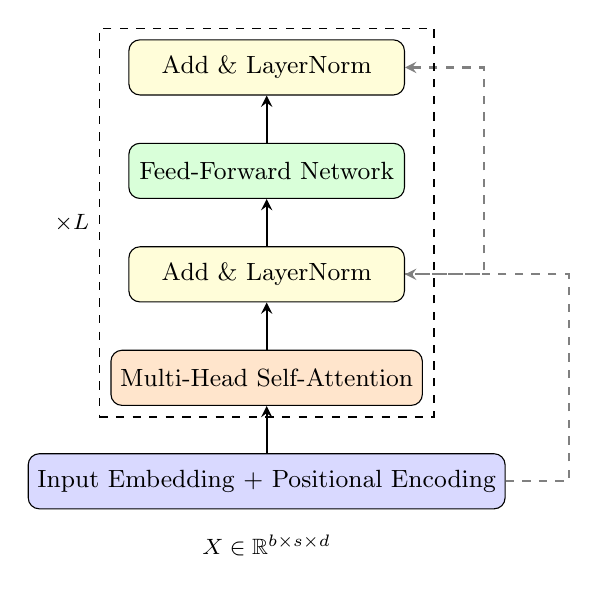
\begin{tikzpicture}[
    node distance=0.6cm,
    box/.style={rectangle, draw, rounded corners, minimum width=3.5cm, minimum height=0.7cm, align=center, font=\small},
    arrow/.style={->, >=stealth, thick},
]

% Encoder
\node[box, fill=blue!15] (emb) {Input Embedding + Positional Encoding};
\node[box, fill=orange!20, above=of emb] (mha) {Multi-Head Self-Attention};
\node[box, fill=yellow!15, above=of mha] (add1) {Add \& LayerNorm};
\node[box, fill=green!15, above=of add1] (ffn) {Feed-Forward Network};
\node[box, fill=yellow!15, above=of ffn] (add2) {Add \& LayerNorm};

\draw[arrow] (emb) -- (mha);
\draw[arrow] (mha) -- (add1);
\draw[arrow] (add1) -- (ffn);
\draw[arrow] (ffn) -- (add2);

% Residual connections
\draw[arrow, dashed, gray] (emb.east) -- ++(0.8,0) |- (add1.east);
\draw[arrow, dashed, gray] (add1.east) -- ++(1.0,0) |- (add2.east);

% Label
\node[draw, dashed, fit=(mha)(add1)(ffn)(add2), inner sep=4pt, label={[font=\footnotesize]left:$\times L$}] {};
\node[below=0.2cm of emb, font=\footnotesize\itshape] {$X \in \mathbb{R}^{b \times s \times d}$};

\end{tikzpicture}
\caption{Transformer encoder block. The block repeats $L$ times. Under tensor parallelism, the multi-head attention and FFN layers are sharded across GPUs, requiring AllReduce communication after each.}
\label{fig:transformer-block}
\end{figure}

For distributed inference, the critical observation is that each transformer layer produces activation tensors of shape $(b, s, d_{\text{model}})$ that must be communicated between pipeline stages, and KV cache tensors of shape $(b, h, s, d_k)$ per layer that accumulate during generation.

\subsection{FlashAttention Evolution}

The standard attention computation has $O(s^2)$ memory complexity due to materializing the $s \times s$ attention matrix. For long sequences ($s = 8192$ or higher), this becomes the dominant memory bottleneck.

\textbf{FlashAttention}~\cite{dao2022flashattention} introduced IO-aware tiling that computes attention in blocks, keeping the working set in GPU SRAM rather than HBM. By avoiding the materialization of the full attention matrix, FlashAttention achieves exact attention with $O(s)$ memory and 2--4$\times$ wall-clock speedup on GPT-2 training.

\begin{figure}[htbp]
\centering
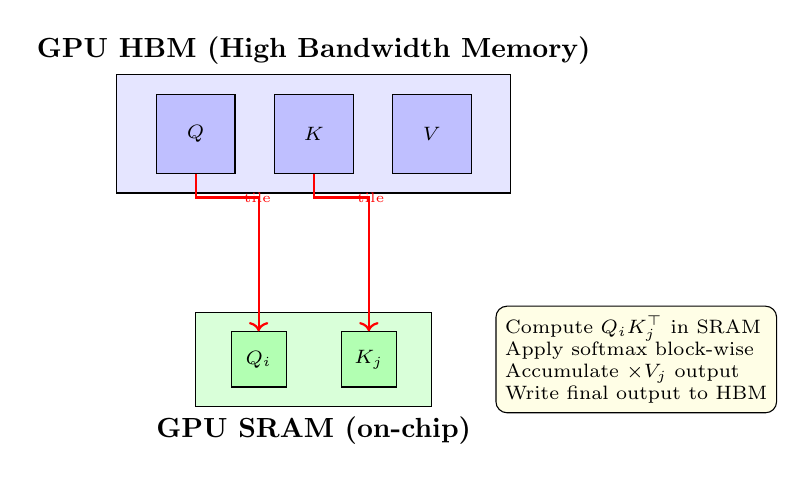
\begin{tikzpicture}[
    node distance=0.4cm,
    block/.style={rectangle, draw, minimum width=1cm, minimum height=1cm, align=center, font=\scriptsize},
]

% HBM
\node[draw, minimum width=5cm, minimum height=1.5cm, fill=blue!10, label={above:\textbf{GPU HBM (High Bandwidth Memory)}}] (hbm) at (0,0) {};
\node[block, fill=blue!25] (q) at (-1.5,0) {$Q$};
\node[block, fill=blue!25] (k) at (0,0) {$K$};
\node[block, fill=blue!25] (v) at (1.5,0) {$V$};

% SRAM
\node[draw, minimum width=3cm, minimum height=1.2cm, fill=green!15, below=1.5cm of hbm, label={below:\textbf{GPU SRAM (on-chip)}}] (sram) {};
\node[block, fill=green!30, minimum width=0.7cm, minimum height=0.7cm] (qt) at ($(sram.center)+(-0.7,0)$) {$Q_i$};
\node[block, fill=green!30, minimum width=0.7cm, minimum height=0.7cm] (kt) at ($(sram.center)+(0.7,0)$) {$K_j$};

% Arrows
\draw[->, thick, red] (q.south) -- ++(0,-0.3) -| (qt.north) node[pos=0.3, right, font=\tiny] {tile};
\draw[->, thick, red] (k.south) -- ++(0,-0.3) -| (kt.north) node[pos=0.3, right, font=\tiny] {tile};

% Annotation
\node[draw, rounded corners, fill=yellow!10, right=0.8cm of sram, minimum width=2.5cm, align=left, font=\scriptsize] {
    Compute $Q_iK_j^\top$ in SRAM\\
    Apply softmax block-wise\\
    Accumulate $\times V_j$ output\\
    Write final output to HBM
};

\end{tikzpicture}
\caption{FlashAttention tiling. Instead of materializing the full $s \times s$ attention matrix in HBM, FlashAttention loads tiles of $Q$ and $K$ into SRAM, computes partial attention, and accumulates results incrementally.}
\label{fig:flashattention-tiling}
\end{figure}

\textbf{FlashAttention-2}~\cite{dao2023flashattention2} improved parallelism by partitioning work across warps within a thread block, achieving 50--73\% of peak FLOPs on A100 GPUs. The key insight is reducing synchronization between warps by assigning non-overlapping rows of the output matrix to different warps.

\textbf{FlashAttention-3}~\cite{shah2024flashattention3} targets Hopper (H100) and Blackwell architectures, exploiting hardware asynchrony between tensor cores, memory loads, and softmax computation. It introduces FP8 quantization for the $QK^\top$ computation, achieving 740~TFLOPs/s on H100---1.5--2$\times$ faster than FA2. Section~\ref{sec:fa3-fix} documents our fix enabling FA3 on Blackwell (RTX~5090) GPUs.

\subsection{PagedAttention}

Kwon et al.~\cite{kwon2023pagedattention} observed that KV cache memory in serving systems is severely fragmented: each request reserves contiguous memory for its maximum possible sequence length, wasting 60--80\% of allocated KV memory. PagedAttention applies the operating system concept of virtual memory paging to KV cache management.

KV cache is divided into fixed-size blocks (e.g., 16 tokens per block). A block table maps logical token positions to physical memory blocks, enabling non-contiguous storage. This achieves near-zero waste and enables memory sharing across requests with common prefixes.

PagedAttention's block-based KV cache is precisely what our RDMA middleware transfers between GPUs. The block granularity (typically 16--64 tokens $\times$ $d_{\text{head}}$ $\times$ 2 bytes $=$ 2--16~KB per block) maps well to RDMA transfer sizes where the NIC can achieve high throughput without excessive protocol overhead.

\subsection{GPU Architecture Evolution: From Graphics to Inference}
\label{sec:tensor-core-evolution}

Early NVIDIA GPUs were designed for rasterization and shading---workloads dominated by independent per-pixel computations. These architectures excelled at vision tasks (image classification, object detection) because convolutional neural networks exhibit the same per-element parallelism: each pixel's convolution kernel operates independently, mapping naturally onto thousands of CUDA cores executing identical instructions across different data (SIMT). The bottleneck was compute throughput, not data movement.

Modern LLM inference inverts this relationship. Autoregressive token generation is inherently sequential (each token depends on the previous token's KV cache), the attention mechanism requires dense matrix-matrix multiplications across the entire context window, and the dominant cost shifts from FLOPs to memory bandwidth~\cite{patel2025tensorcore}. This architectural mismatch drove NVIDIA to redesign GPU hardware from the transistor level upward, evolving Tensor Cores across five generations to match the compute patterns of transformer workloads.

\subsubsection{Volta: 1st Generation Tensor Cores (2017)}

Volta (V100) introduced the first Tensor Cores, purpose-built Matrix-Multiply-Accumulate (MMA) units that operate on FP16 inputs with FP32 accumulation~\cite{patel2025tensorcore}. Each Tensor Core computes a $4 \times 4 \times 4$ fused multiply-add per cycle. The MMA instruction is \emph{warp-scoped}: a warp of 32 threads collectively feeds an $8 \times 8 \times 4$ matrix tile (shape \texttt{m8n8k4}) to the Tensor Cores, producing 1,024 FP16 FLOPs per cycle per SM.

Volta's Tensor Cores delivered an order-of-magnitude improvement over CUDA cores for matrix operations, but they support only FP16 input $\to$ FP32 accumulate. Our V100 GPUs in Tower~2 inherit this limitation: tensors must be in IEEE FP16 format before Tensor Core execution. BF16 is not supported in hardware, which creates the precision mismatch with the RTX~5070~Ti (BF16-native) that motivates the RDMA Tensor Cache's stochastic rounding pipeline (Section~\ref{sec:neumann-integration}).

\subsubsection{Turing and Ampere: Expanding Precision Support}

Turing (2nd generation, 2018) added INT8 and INT4 Tensor Core paths, enabling efficient inference quantization. Ampere (3rd generation, A100, 2020) expanded further with BF16 support and \texttt{ldmatrix}---an instruction that loads a warp-wide matrix tile from shared memory into registers in a single operation. Ampere also introduced \emph{asynchronous data copies} (\texttt{cp.async}), decoupling global-to-shared memory transfers from compute~\cite{patel2025tensorcore}. The MMA scope widened from warp-scoped to \emph{warp-level synchronous}: the \texttt{mma.sync} instruction operates at the warp level with shape \texttt{m16n8k16}, doubling throughput to 2,048 FP16 FLOPs/cycle/SM. Ampere also introduced \emph{2:4 structured sparsity}, which prunes 2 of every 4 weight elements, theoretically doubling Tensor Core throughput by halving the work.

\subsubsection{Hopper: Asynchronous Everything}

Hopper (H100, 4th generation, 2022) fundamentally restructured the GPU memory hierarchy for LLM workloads with three innovations~\cite{patel2025tensorcore}:

\begin{enumerate}
    \item \textbf{Thread Block Clusters:} A new hierarchy level where multiple CTAs (Cooperative Thread Arrays) across different SMs form a cluster. CTAs within a cluster can access each other's shared memory via \emph{Distributed Shared Memory} (DSMEM), enabling cross-SM data sharing without going through L2 cache or HBM.

    \item \textbf{Tensor Memory Accelerator (TMA):} A hardware unit that handles multi-dimensional tensor addressing and data movement between global memory and shared memory. TMA supports \emph{multicast loads}: a single instruction loads data from global memory into the shared memory of multiple SMs simultaneously, reducing L2 cache traffic and HBM bandwidth consumption. However, TMA has higher latency than regular \texttt{cp.async} for small transfers (due to address generation overhead), making it best suited for large, regular data movements rather than small KV cache page loads~\cite{patel2025tensorcore}.

    \item \textbf{Warpgroup-level Asynchronous MMA (\texttt{wgmma}):} The MMA scope expands again---a warpgroup of 4 warps (128 threads) collectively performs one MMA operation. \texttt{wgmma} reads operand~A from registers or shared memory and operand~B exclusively from shared memory, reducing register pressure. The shape expands to \texttt{m64nNk16} where N ranges from 8 to 256, yielding 4,096 FP16 FLOPs/cycle/SM. Critically, Hopper introduces FP8 (E4M3 and E5M2) Tensor Core paths with FP32 accumulation---though the accumulation path is actually a 22-bit fixed-point format (13-bit mantissa), requiring periodic writeback to CUDA cores for full-precision accumulation~\cite{patel2025tensorcore}.
\end{enumerate}

FlashAttention-3~\cite{shah2024flashattention3} exploits all three Hopper features: TMA for asynchronous $Q/K/V$ tile loads, \texttt{wgmma} for the attention matrix multiply, and DSMEM for cross-SM $K/V$ sharing during multi-query attention. This achieves 740~TFLOPs/s (1.5--2$\times$ over FA2)---demonstrating that the memory system is now the primary bottleneck, not the Tensor Cores themselves.

\subsubsection{Blackwell: Tensor Memory and Cross-SM Fusion}

Blackwell (GB100/GB200, 5th generation, 2024) targets inference-at-scale with two architectural departures~\cite{patel2025tensorcore}:

\begin{enumerate}
    \item \textbf{Tensor Memory (TMEM):} A new 256~KB memory per SM, dedicated to Tensor Core operands. TMEM has 128 rows (lanes) $\times$ 512 columns of 4-byte cells, with a restricted access pattern: a warpgroup of 4 warps collectively accesses the full TMEM, each warp owning 32 lanes. By limiting access patterns, NVIDIA reduces access port count and chip area. Unlike shared memory, TMEM must be explicitly managed by the programmer (allocation, deallocation, copy-in/copy-out).

    \item \textbf{5th Generation MMA (\texttt{tcgen05.mma}):} The MMA instruction moves to \emph{single-thread semantics}---a single thread issues the MMA, reading operand~A and writing output~D to TMEM, while reading operand~B from shared memory. This eliminates the complex register-to-Tensor-Core data layouts of previous generations and frees thread registers for other work (epilogue operations like activation functions). A notable variant, \texttt{MMA.2SM}, fuses two SMs in a CTA pair (mapped to a Texture Processing Cluster) to collectively perform a single larger MMA, doubling the M dimension to \texttt{m256nNk16} and halving the B-matrix loads via DSMEM sharing between the paired SMs.
\end{enumerate}

Blackwell doubles Tensor Core throughput to 8,192 FP16 FLOPs/cycle/SM across 148 SMs, with 186~GB HBM3e at 8,000~GB/s. It adds native MXFP8, MXFP6, and MXFP4 microscaling format support~\cite{rouhani2023mxfp4}, plus NVIDIA's proprietary NVFP4 format which uses smaller block sizes and two-level quantization for higher accuracy than standard MXFP4.

\begin{table}[htbp]
\centering
\caption{Tensor Core architecture evolution across GPU generations~\cite{patel2025tensorcore}. Each generation shifts the bottleneck further from compute to memory bandwidth, motivating RDMA optimization.}
\label{tab:tensorcore-evolution}
\small
\begin{tabular}{@{}lcccc@{}}
\toprule
& \textbf{Volta (V100)} & \textbf{Ampere (A100)} & \textbf{Hopper (H100)} & \textbf{Blackwell (GB200)} \\
\midrule
Generation & 1st & 3rd & 4th & 5th \\
SMs & 80 & 108 & 132 & 148 \\
FP16 FLOPs/cycle/SM & 1,024 & 2,048 & 4,096 & 8,192 \\
HBM Capacity & 16 GB & 40 GB & 80 GB & 186 GB \\
HBM Bandwidth & 900 GB/s & 1,555 GB/s & 3,350 GB/s & 8,000 GB/s \\
L2 Cache & 6 MB & 40 MB & 50 MB & 130 MB \\
Shared Mem / SM & 96 KB & 164 KB & 228 KB & 228 KB \\
MMA Scope & Warp & Warp & Warpgroup & Single Thread \\
FP16 MMA Shape & \texttt{m8n8k4} & \texttt{m16n8k16} & \texttt{m64nNk16} & \texttt{m256nNk16} \\
MMA SASS & HMMA & HMMA & HGMMA & UTCHMMA \\
Lowest Precision & FP16 & INT4 & FP8 (E4M3) & NVFP4 / MXFP4 \\
\bottomrule
\end{tabular}
\end{table}

\subsubsection{Implications for RDMA Tensor Transfers}

The five-generation evolution reveals a consistent trend: NVIDIA scales Tensor Core size (FLOPs per SM) faster than the number of Tensor Cores, because matrix multiplication arithmetic intensity scales cubically ($O(n^3)$ FLOPs) while data movement scales quadratically ($O(n^2)$ reads)~\cite{patel2025tensorcore}. Larger tiles amortize memory latency better. But this means the gap between compute capability and memory bandwidth widens each generation---the GPU can process tensors faster than it can fetch them from HBM, let alone receive them over a network.

For our heterogeneous cluster, this has three direct consequences:
\begin{enumerate}
    \item \textbf{Precision diversity:} The V100 supports only FP16 Tensor Core input; the 5070~Ti (Blackwell-class consumer) supports BF16 and FP8. Every tensor transferred between towers must undergo precision conversion. The RDMA Tensor Cache's FP32 master weights and stochastic rounding pipeline exist precisely because these GPUs cannot share a native precision format.

    \item \textbf{Memory hierarchy depth:} Hopper and Blackwell add DSMEM and TMEM respectively, creating additional levels that tensor data must traverse. RDMA-delivered tensors land in HBM via GPUDirect; efficient kernels must then tile them through L2 $\to$ shared memory $\to$ TMEM/registers before Tensor Cores can consume them. The prefetch FSM (Section~\ref{sec:neumann-integration}) must account for this multi-level pipeline.

    \item \textbf{Transfer size alignment:} Blackwell's \texttt{m256nNk16} tiles are $16\times$ larger than Volta's \texttt{m8n8k4}. RDMA transfer sizes should align with the destination GPU's tile granularity to avoid partial-tile stalls. The WFA classifier's hot/cold categorization implicitly captures this: small, latency-sensitive transfers (KV cache pages matching Volta's smaller tiles) take the hot path, while large weight tiles (matching Blackwell's larger MMA shapes) take the cold path with batching.
\end{enumerate}

%=============================================================================
\section{Scheduling, Scaling, and Expert Parallelism}
\label{sec:scheduling-scaling}
%=============================================================================

\subsection{Scheduling Algorithms for Tensor Transfers}
\label{sec:gpu-scheduling}

Efficient scheduling of tensor transfers across an RDMA fabric requires algorithms that overlap communication with computation and respect data dependencies. The problem is structurally analogous to GPU cluster scheduling, where jobs with heterogeneous resource demands and interdependencies must be assigned to accelerators with minimal idle time. Chab et al.~\cite{gpu-scheduling-survey} provide a comprehensive taxonomy of GPU scheduling algorithms organized into four algorithmic families---classical optimization, queueing-theoretic, learning-based, and hybrid---each with distinct applicability to tensor transfer scheduling.

\subsubsection{Classical Optimization Algorithms}

Classical schedulers rely on deterministic rules or mathematical optimization without any learning component~\cite{gpu-scheduling-survey}. The simplest are \emph{greedy algorithms}: Shortest-Job-First (SJF) processes the job with the smallest expected runtime next, minimizing average completion time on a single GPU. For tensor transfers, this maps to prioritizing small, latency-sensitive tensors (KV cache pages, attention scores) over large bulk transfers (gradient accumulations)---the same intuition behind our hot/cold path differentiation. However, SJF can starve large transfers indefinitely; production systems mitigate this with \emph{aging} policies that promote long-waiting transfers to higher priority~\cite{tiresias2019}.

\emph{Backfilling} extends FCFS by allowing smaller transfers to leapfrog the head-of-queue when resources are idle, while reserving capacity for the blocked head transfer. In RDMA terms, small KV cache reads can proceed on available Queue Pairs while a large gradient AllReduce waits for all QPs in its group. First-Fit (FF) and Best-Fit (BF) packing heuristics reduce multi-GPU placement to a bin-packing problem; on \emph{heterogeneous} clusters like ours (V100 + 5070~Ti), Gavel~\cite{gavel2020} normalizes job throughput across GPU types by scheduling in the transformed space of \emph{effective GPU-seconds}, extending classical packing heuristics to handle device heterogeneity while preserving fairness.

\emph{Dynamic programming (DP)} computes exact schedules for small problem instances. Production GPU schedulers often embed DP selectively: OASiS uses polynomial-time DP inside an online primal-dual algorithm to determine high-priority worker/parameter-server allocations, achieving near-optimal throughput with per-decision latencies below 100~ms~\cite{gpu-scheduling-survey}. For RDMA tensor scheduling, a lightweight DP could optimize the assignment of tensor batches to QPs within a single scheduling epoch.

\emph{ILP/MILP formulations} provide provably optimal schedules but are computationally expensive (NP-hard even for $m=2$ GPUs~\cite{gpu-scheduling-survey}). MILP is practical for offline calibration---computing optimal QP assignments for a fixed model architecture---then deploying the resulting allocation table at runtime.

\emph{Meta-heuristics} (genetic algorithms, simulated annealing, Tabu search) explore large search spaces but require seconds to minutes per schedule, making them unsuitable for online tensor scheduling. They remain useful for offline parameter tuning: running a GA on historical traces to optimize scheduling-policy weights, then deploying the tuned heuristic for real-time decisions.

\subsubsection{Queueing-Theoretic Approaches}

Queueing-theoretic schedulers assign each tensor transfer a dynamic priority based on its service history, rather than solving a global optimization~\cite{gpu-scheduling-survey}. \emph{Index policies} compute a per-transfer score that balances fairness and efficiency. The Gittins index is a canonical example for $M/G/1$ queues: a transfer with attained service $v$ receives a priority score that rewards transfers likely to complete soon. While exact computation is complex, approximations yield near-optimal mean-slowdown performance when transfer sizes are unknown.

\emph{Least Attained Service (LAS)} always runs the transfer with the smallest accumulated service time, achieving at most 25\% penalty over SRPT for mean slowdown under heavy-tailed distributions~\cite{gpu-scheduling-survey}. Tiresias~\cite{tiresias2019} adapts LAS to GPU clusters using two-dimensional LAS (2D-LAS) that tracks both time and GPU count, preempting transfers with fixed-length leases rather than costly full preemption. E-LAS extends this by incorporating real-time epoch progress rates. For RDMA tensor transfers, a LAS-inspired policy would track cumulative bytes transferred per tensor stream and prioritize streams with the least accumulated transfer volume---naturally favoring small, infrequent transfers (KV cache) over bulk data (weights).

\emph{Multi-class priority queues} divide transfers into priority classes---``hot'' for latency-critical KV cache and attention tensors, ``warm'' for pipeline activations, ``cold'' for bulk gradient and weight transfers. Strict priority in an $M/M/1$ system guarantees minimal response for the hot class, though cold transfers may experience increased delays~\cite{gpu-scheduling-survey}. Our WFA classifier (Section~\ref{sec:architecture}) implements exactly this pattern, with learned transition weights that adapt class boundaries to workload phase (prefill vs.\ decode).

\emph{Predictive admission control} uses queueing theory formulas to drive service-level guarantees. Little's Law ($L = \lambda W$), mean response-time bounds, and $M/M/1$ approximations can trigger autoscaling of RDMA QPs or more aggressive preemption when congestion looms---directly relevant to our RoCE timeout mitigation (Section~\ref{sec:critical-issues}).

\subsubsection{Learning-Based Adaptive Algorithms}

Learning-based schedulers harness machine learning to adapt scheduling policies from data~\cite{gpu-scheduling-survey}. \emph{Supervised prediction models} are trained on job features to forecast metrics like runtime, memory footprint, or scaling behavior. A scheduler then implements data-driven SJF by ordering transfers according to predicted completion times. In heterogeneous GPU clusters, Gavel~\cite{gavel2020} benchmarks workloads to derive throughput estimates for different GPU types, adapting classical policies to mixed environments.

\emph{Reinforcement learning (RL)} casts scheduling as a sequential decision problem. DeepRM~\cite{deeprm2016} encodes the cluster as an image of resource occupancy and trains a neural network to output scheduling distributions. Decima~\cite{decima2019} extends this with graph neural networks that embed DAG-structured workloads, outperforming heuristics like SRTF under variable load. HeterPS applies LSTM-based RL to allocate tasks across CPUs and GPUs in heterogeneous clusters~\cite{gpu-scheduling-survey}.

RL faces four practical challenges for production deployment~\cite{gpu-scheduling-survey}: (1) \emph{exploration vs.\ exploitation}---suboptimal actions during training can degrade live performance; (2) \emph{state-space explosion}---real clusters with hundreds of concurrent transfers exceed tractable state representations; (3) \emph{stability and safety}---unconstrained RL policies may starve critical transfers or violate SLOs; and (4) \emph{interpretability}---opaque policies hinder debugging in mission-critical environments. Hybrid designs address these by combining learned models for parameter tuning with proven rule-based control logic for the primary decision path.

\emph{Adaptive scheduling via feedback control} continuously monitors system metrics and adjusts scheduling behavior in a closed loop~\cite{gpu-scheduling-survey}. Pollux~\cite{pollux2021} uses online goodput feedback per job to dynamically adjust GPU allocations: if additional GPUs do not improve goodput (diminishing returns), the system reduces that job's share and reallocates to others. AntMan similarly modifies deep learning frameworks for fine-grained, real-time scaling of GPU memory and compute without requiring job restarts. For RDMA tensor scheduling, a feedback-driven approach would monitor transfer completion rates, QP queue depths, and congestion signals (ECN marks, RTT variance), then adjust hot/cold thresholds and QP allocation dynamically.

\subsubsection{Comparative Analysis and Applicability}

Chab et al.~\cite{gpu-scheduling-survey} evaluate scheduling algorithm families across four dimensions. We summarize the key trade-offs relevant to tensor transfer scheduling:

\begin{table}[htbp]
\centering
\caption{Comparative analysis of GPU scheduling algorithm families~\cite{gpu-scheduling-survey} and their applicability to RDMA tensor scheduling}
\label{tab:scheduling-comparison}
\footnotesize
\resizebox{\textwidth}{!}{%
\begin{tabular}{@{}p{2cm}p{1.8cm}p{2cm}p{2cm}p{3.2cm}@{}}
\toprule
\textbf{Family} & \textbf{Decision Speed} & \textbf{Schedule Quality} & \textbf{Heterogeneity} & \textbf{RDMA Tensor Application} \\
\midrule
Greedy / Heuristic & $O(\log n)$, sub-ms & Good avg., no worst-case bounds & Extensible (Gavel) & Hot/cold QP assignment, backfill for small KV transfers \\
ILP / MILP & Seconds--minutes & Provably optimal & Via constraints & Offline QP allocation calibration \\
Queueing-Theoretic & $O(1)$ per-job index & Near-optimal fairness (Gittins) & Per-resource queues & LAS-based transfer prioritization, admission control \\
Learning-Based (RL) & ms (inference) & Near-optimal (trained) & Encoded in state & Adaptive threshold tuning, congestion prediction \\
Hybrid & ms (heuristic) + periodic optimization & Strong practical & Flexible & WFA classifier + periodic QP rebalancing \\
\bottomrule
\end{tabular}%
}
\end{table}

The survey identifies that no single paradigm dominates across all scenarios. \emph{Offline deterministic} workloads favor ILP/DP for optimal schedules. \emph{Online workloads with heavy-tailed transfer sizes}---typical of LLM inference where KV cache transfers are small and frequent while gradient syncs are large and periodic---benefit from queueing-theoretic policies like LAS or Gittins that balance fairness and mean response time. \emph{Heterogeneous resources} (our V100+5070~Ti cluster) require two-stage approaches: first matching transfers to resource classes, then applying standard scheduling within each class~\cite{gavel2020}. \emph{Multi-tenant cloud environments} demand fairness mechanisms; Themis~\cite{themis2020} uses partial-auction frameworks supplemented by SJF inner loops.

Production systems converge on \emph{hybrid strategies}: lightweight heuristics for real-time dispatch, ILP or matching solvers for small-scale assignment tasks, and learning models for runtime and resource-usage prediction~\cite{gpu-scheduling-survey}. Our middleware adopts this hybrid pattern: the WFA classifier provides the heuristic real-time dispatch (hot/warm/cold in $O(1)$), periodic telemetry analysis provides the optimization feedback loop, and the prefetch engine's pattern classifier (Section~\ref{sec:neumann-integration}) provides the learned prediction component.

\subsubsection{Mapping to RDMA Tensor Scheduling}

We additionally draw analogies from quantum circuit scheduling~\cite{zhong2025quantum}, where three algorithmic patterns map to RDMA tensor transfer optimization:

\begin{table}[htbp]
\centering
\caption{Scheduling algorithm mapping from quantum/GPU domains to RDMA tensor transfers}
\label{tab:scheduling-mapping}
\footnotesize
\resizebox{\textwidth}{!}{%
\begin{tabular}{@{}p{2.5cm}p{2.2cm}p{4cm}p{2.2cm}@{}}
\toprule
\textbf{Scheduling Concept} & \textbf{Original Domain} & \textbf{RDMA Tensor Application} & \textbf{WFA State} \\
\midrule
BBOP (Batch-Buffered Overlap) & Quantum circuit gate batching & Batch cold-path tensor transfers; overlap with hot-path RDMA writes & Cold $\to$ Batched \\
SMGP (Staggered Multi-Gate Parallelism) & Parallel quantum gate execution & Pipeline-parallel activation overlap; stagger layer transfers across QPs & Warm $\to$ Pipelined \\
DAGC (Dependency-Aware Gate Contraction) & Circuit DAG optimization & WFA-driven tensor coalescing; merge adjacent cold tensors into single RDMA write & Cold $\to$ Coalesced \\
Priority-based scheduling~\cite{gpu-scheduling-survey} & GPU job scheduling & Hot/cold path differentiation; dedicated QPs for latency-critical tensors & Hot $\to$ Priority QP \\
Preemptive scheduling~\cite{gpu-scheduling-survey} & OS process scheduling & Tensor reclassification during phase changes (prefill $\to$ decode) & State transition \\
Feedback-driven scaling~\cite{pollux2021} & GPU goodput optimization & Monitor QP queue depth; adjust hot/cold thresholds via telemetry & Adaptive $\to$ Rebalance \\
\bottomrule
\end{tabular}%
}
\end{table}

The BBOP pattern is particularly relevant: during training, gradient tensors from completed layers can be batched into a single RDMA transfer while the next layer's forward pass proceeds. The prefetch engine (Section~\ref{sec:neumann-integration}) implements a variant of SMGP by issuing speculative RDMA reads for upcoming layers while the current layer computes. The feedback-driven approach from Pollux~\cite{pollux2021} informs our telemetry-based QP rebalancing: monitoring transfer completion rates per QP and reallocating capacity from underutilized cold-path channels to congested hot-path channels.

The survey's analysis of \emph{practical integration challenges}---resource-manager interfacing, distributed workload coordination, framework coupling, GPU-specific APIs, scheduler overhead, preemption cost, and monitoring overhead~\cite{gpu-scheduling-survey}---directly applies to our middleware. Our transport abstraction layer addresses framework coupling by providing a stable interface across vLLM, exo, and custom training loops. The container-aware communication broker (Section~\ref{sec:critical-issues}) addresses the deployment challenges that Chab et al.\ identify as a gap between algorithmic elegance and engineering practicality.

\subsection{Mixture of Experts}

Mixture-of-Experts (MoE) models use conditional computation to increase model capacity without proportionally increasing compute. GShard~\cite{lepikhin2020gshard} introduced expert parallelism for distributed MoE training, where experts are distributed across GPUs and a gating network routes each token to its top-$k$ experts.

The Switch Transformer~\cite{fedus2021switch} simplified this to top-1 routing: each token is sent to exactly one expert, reducing the communication overhead from $O(k \cdot E)$ to $O(E)$ AllToAll messages. With $E$ experts distributed across $N$ GPUs, each GPU hosts $E/N$ experts and must exchange tokens with all other GPUs via AllToAll. DeepSeek-V3~\cite{deepseekv3} scaled this to 671B total parameters (37B activated per token) using Multi-head Latent Attention and an auxiliary-loss-free load balancing strategy, training on 14.8T tokens in 2.788M H800 GPU hours---demonstrating that MoE architectures with adaptive routing are the dominant paradigm for cost-efficient frontier models.

Expert parallelism interacts with tensor and data parallelism through:
\begin{equation}
    \texttt{EP\_SIZE} = \texttt{TP} \times \texttt{DP}
\end{equation}
as documented in the AMD ROCm guide~\cite{amd-moe-guide}. The AllToAll communication pattern is inherently asymmetric---different tokens route to different experts, creating variable-size messages---which makes it particularly amenable to adaptive routing. Hot experts (those receiving many tokens) generate larger, more frequent transfers that benefit from priority QP assignment.

\subsection{Scaling Laws and the Communication Bottleneck}

Kaplan et al.~\cite{kaplan2020scaling} established power-law relationships between model size, dataset size, compute budget, and loss. For a model with $N$ parameters trained on $D$ tokens with compute budget $C$:
\begin{equation}
    L(N) \propto N^{-0.076}, \quad L(D) \propto D^{-0.095}, \quad L(C) \propto C^{-0.050}
\end{equation}

Hoffmann et al.~\cite{hoffmann2022chinchilla} refined this with the Chinchilla scaling law: for compute-optimal training, a model with $N$ parameters should be trained on approximately $20N$ tokens. This implies that as models grow from 7B to 70B to 700B parameters, training data scales proportionally, and the communication overhead of distributing both model and data across GPUs grows superlinearly.

For a model distributed across $P$ GPUs with tensor parallelism degree $T$, the per-layer AllReduce volume is:
\begin{equation}
    V_{\text{AllReduce}} = 2 \cdot b \cdot s \cdot d \cdot \frac{T-1}{T}
\end{equation}
and the total communication per training step scales as $O(L \cdot b \cdot s \cdot d)$, where $L$ is the number of layers. For a 70B model ($L=80$, $d=8192$) with batch size 32 and sequence length 4096, this is approximately 172~GB per step---saturating a 100GbE link for over 13 seconds if not overlapped with computation. This makes RDMA optimization increasingly critical as models scale.

%=============================================================================
\section{RDMA Fundamentals and the Communication Bottleneck}
\label{sec:rdma-fundamentals}
%=============================================================================

\subsection{RDMA Programming Model}

The RDMA programming model~\cite{infiniband-rdma} provides three key abstractions that our transport layer mirrors:

\begin{enumerate}
    \item \textbf{Memory Registration:} Before RDMA operations, memory regions must be registered with the NIC via \texttt{ibv\_reg\_mr}. This pins physical pages and provides the NIC with a translation table. Registration is expensive ($\sim$10~$\mu$s) but amortized across thousands of RDMA operations on the same buffer.

    \item \textbf{Queue Pairs (QPs):} Communication endpoints consisting of a Send Queue and Receive Queue. Reliable Connection (RC) QPs provide guaranteed delivery with retransmission; Dynamic Connection (DC) QPs multiplex a single QP across peers, scaling to $O(1)$ rather than $O(n^2)$ state for $n$-node clusters.

    \item \textbf{One-Sided Operations:} RDMA Read and Write execute without involving the remote CPU. The initiating NIC issues the DMA directly to/from the remote NIC, which accesses the pre-registered memory region. This is why GPUDirect RDMA is so effective: the NIC writes directly into GPU BAR1 memory, bypassing both CPUs entirely.
\end{enumerate}

For a tensor of size $S$ bytes, the total transfer time over RDMA is:
\begin{equation}
    T_{\text{RDMA}} = T_{\text{latency}} + \frac{S}{B_{\text{link}}} + T_{\text{DMA}}
\end{equation}
where $T_{\text{latency}}$ is the one-way latency ($\sim$2~$\mu$s for hardware RoCE), $B_{\text{link}}$ is the link bandwidth (12.5~GB/s for 100GbE), and $T_{\text{DMA}}$ is the DMA engine overhead ($\sim$0.5~$\mu$s). For a 256~MB gradient tensor, $T_{\text{RDMA}} \approx 2 + 20480 + 0.5 \approx 20.5$~ms---dominated by bandwidth, confirming that 100GbE is the bottleneck rather than RDMA protocol overhead.

\subsection{The Communication Bottleneck}

Current distributed ML systems suffer from a fundamental mismatch: NCCL~\cite{nccl} employs static routing strategies optimized for bulk transfers, creating head-of-line (HOL) blocking where small, latency-sensitive tensors (KV cache pages, attention scores) wait behind large bulk transfers (model weights, gradient accumulations). NCCL discovers network topology at initialization but does not adapt routing based on runtime access patterns.

This manifests in two ways:
\begin{enumerate}
    \item \textbf{Inference:} Time-To-First-Token (TTFT) latency increases because KV cache transfers share the same communication channel as model weight distribution.
    \item \textbf{Training:} Gradient synchronization delays propagate through the pipeline, reducing GPU utilization from the theoretical maximum.
\end{enumerate}

\subsection{Transport Technologies}

The middleware supports multiple transport backends with different performance characteristics:

\begin{table}[htbp]
\centering
\caption{Transport technology comparison for AI workloads}
\label{tab:transport-comparison}
\begin{tabular}{@{}lcccc@{}}
\toprule
\textbf{Transport} & \textbf{Latency} & \textbf{Throughput} & \textbf{Hardware} & \textbf{Maturity} \\
\midrule
InfiniBand HDR & $<$1 $\mu$s & 200 Gb/s & Dedicated fabric & Production \\
RoCEv2 & 2--5 $\mu$s & 400 Gb/s & ConnectX + DCB & Production \\
Tesla TTPoe~\cite{ttpoe-hotchips} & 1--2 $\mu$s & 100 Gb/s & Commodity Ethernet & Production \\
OCP Falcon~\cite{ocp-falcon} & $\sim$3.5 $\mu$s & 400 Gb/s & Open spec & Emerging \\
UEC 1.0~\cite{uec2025} & $\sim$1.8 $\mu$s & 1.6 Tb/s & Next-gen Ethernet & Emerging \\
Soft-RoCE & $\sim$190 $\mu$s & $<$1 Gb/s & Any NIC & Deprecated \\
\bottomrule
\end{tabular}
\end{table}

TTPoe~\cite{ttpoe-repo} is a lossy protocol that expects packet loss and handles retries locally, eliminating the Priority Flow Control (PFC) requirements that make RoCE fragile. UEC~1.0 is relevant because Mellanox ConnectX NICs are expected to receive UEC firmware updates, meaning our ConnectX-4 hardware may gain UEC support without NIC replacement.

%=============================================================================
% THESIS BODY --- Sections 5--12 (merged from existing updates)
%=============================================================================

%=============================================================================
\section{Problem Statement and Contributions}
\label{sec:problem-statement}
%=============================================================================

\subsection{The Multi-Standard Fragmentation Crisis}

Modern distributed machine learning infrastructure operates across incompatible communication layers designed independently for different hardware ecosystems. As shown in \Cref{fig:fragmentation-overview}, applications must navigate at least five distinct communication paths depending on hardware configuration, with no unified abstraction that preserves performance while enabling portability.

\begin{figure}[htbp]
\centering
\resizebox{\textwidth}{!}{%
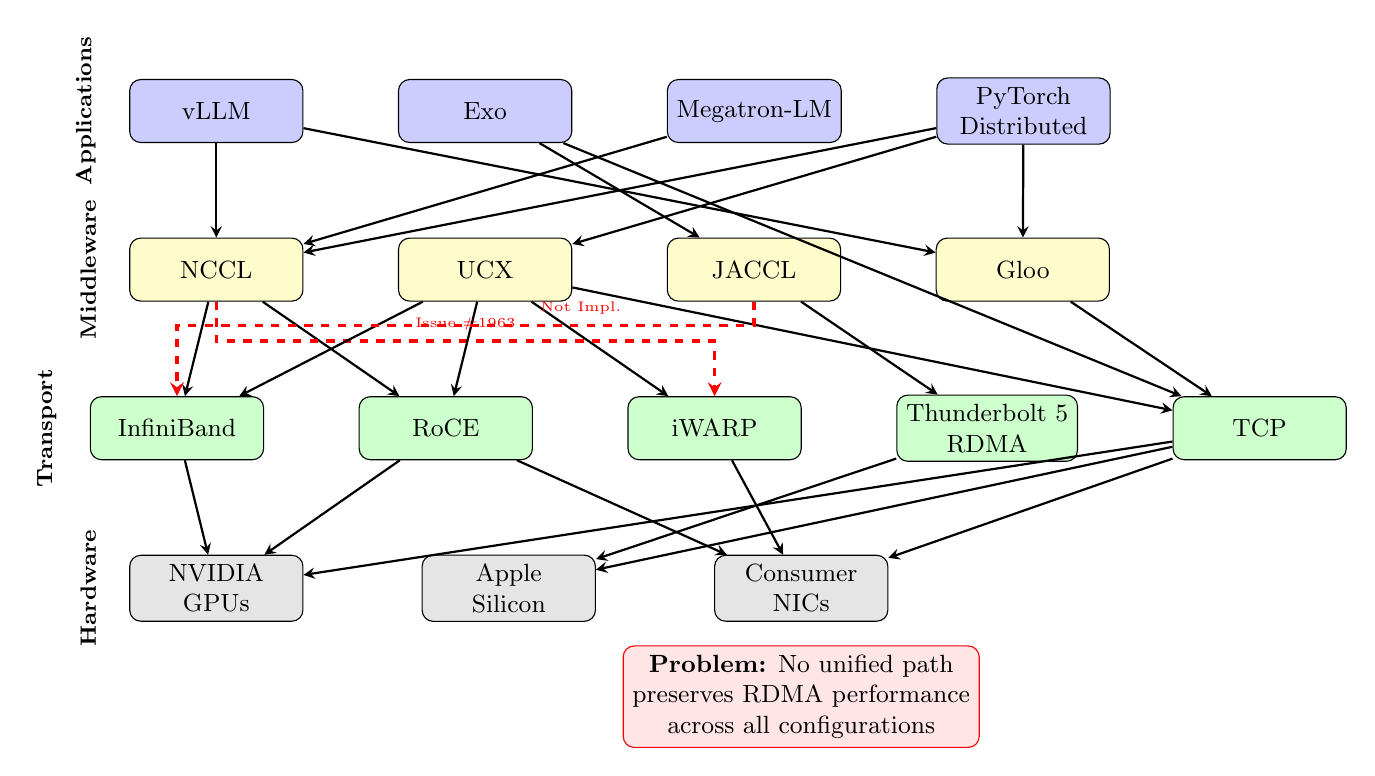
\begin{tikzpicture}[
    node distance=0.8cm and 1.2cm,
    box/.style={rectangle, draw, rounded corners, minimum width=2.2cm, minimum height=0.8cm, align=center, font=\small},
    app/.style={box, fill=blue!20},
    mid/.style={box, fill=yellow!20},
    trans/.style={box, fill=green!20},
    hw/.style={box, fill=gray!20},
    broken/.style={draw=red, very thick, dashed},
    arrow/.style={->, >=stealth, thick}
]

\node[app] (vllm) {vLLM};
\node[app, right=of vllm] (exo) {Exo};
\node[app, right=of exo] (megatron) {Megatron-LM};
\node[app, right=of megatron] (pytorch) {PyTorch\\Distributed};

\node[mid, below=1.2cm of vllm] (nccl) {NCCL};
\node[mid, right=of nccl] (ucx) {UCX};
\node[mid, right=of ucx] (jaccl) {JACCL};
\node[mid, right=of jaccl] (gloo) {Gloo};

\node[trans, below=1.2cm of nccl, xshift=-0.5cm] (ib) {InfiniBand};
\node[trans, right=of ib] (roce) {RoCE};
\node[trans, right=of roce] (iwarp) {iWARP};
\node[trans, right=of iwarp] (tb5) {Thunderbolt 5\\RDMA};
\node[trans, right=of tb5] (tcp) {TCP};

\node[hw, below=1.2cm of ib, xshift=0.5cm] (nvidia) {NVIDIA\\GPUs};
\node[hw, right=1.5cm of nvidia] (apple) {Apple\\Silicon};
\node[hw, right=1.5cm of apple] (consumer) {Consumer\\NICs};

\draw[arrow] (vllm) -- (nccl);
\draw[arrow] (vllm) -- (gloo);
\draw[arrow] (exo) -- (jaccl);
\draw[arrow] (exo) -- (tcp);
\draw[arrow] (megatron) -- (nccl);
\draw[arrow] (pytorch) -- (nccl);
\draw[arrow] (pytorch) -- (gloo);
\draw[arrow] (pytorch) -- (ucx);

\draw[arrow] (nccl) -- (ib);
\draw[arrow] (nccl) -- (roce);
\draw[arrow, broken] (nccl.south) -- ++(0,-0.5) -| (iwarp) node[pos=0.25, above, font=\tiny\color{red}] {Issue \#1963};
\draw[arrow] (ucx) -- (ib);
\draw[arrow] (ucx) -- (roce);
\draw[arrow] (ucx) -- (iwarp);
\draw[arrow] (ucx) -- (tcp);
\draw[arrow] (jaccl) -- (tb5);
\draw[arrow, broken] (jaccl.south) -- ++(0,-0.3) -| (ib) node[pos=0.15, above, font=\tiny\color{red}] {Not Impl.};
\draw[arrow] (gloo) -- (tcp);

\draw[arrow] (ib) -- (nvidia);
\draw[arrow] (roce) -- (nvidia);
\draw[arrow] (roce) -- (consumer);
\draw[arrow] (iwarp) -- (consumer);
\draw[arrow] (tb5) -- (apple);
\draw[arrow] (tcp) -- (nvidia);
\draw[arrow] (tcp) -- (apple);
\draw[arrow] (tcp) -- (consumer);

\node[left=0.3cm of vllm, font=\footnotesize\bfseries, rotate=90, anchor=south] {Applications};
\node[left=0.3cm of nccl, font=\footnotesize\bfseries, rotate=90, anchor=south] {Middleware};
\node[left=0.3cm of ib, font=\footnotesize\bfseries, rotate=90, anchor=south] {Transport};
\node[left=0.3cm of nvidia, font=\footnotesize\bfseries, rotate=90, anchor=south] {Hardware};

\node[draw=red, fill=red!10, rounded corners, font=\small, align=center, below=0.3cm of consumer] (problem) {
    \textbf{Problem:} No unified path\\preserves RDMA performance\\across all configurations
};

\end{tikzpicture}%
}
\caption{Current fragmentation in distributed ML communication stacks. Dashed red lines indicate broken or unimplemented paths identified through GitHub issue analysis.}
\label{fig:fragmentation-overview}
\end{figure}

\subsection{Research Objectives}

This thesis contributes:

\begin{enumerate}[label=\textbf{C\arabic*.}]
    \item \textbf{Unified Telemetry Layer:} A monitoring system that instruments tensor transfers to collect access frequency, transfer size distributions, queue depth at RDMA endpoints, and latency percentiles.
    \item \textbf{WFA Tensor Classifier:} A Weighted Finite Automaton that classifies tensors into hot/warm/cold categories based on observed runtime access patterns, enabling intelligent routing.
    \item \textbf{Smart RDMA Routing:} Dual-path routing with dedicated Queue Pairs for latency-sensitive transfers and batched throughput-optimized channels for bulk data.
    \item \textbf{RDMA Tensor Cache:} A centralized precision management layer in the Neumann runtime that resolves FP16/BF16 mismatches across heterogeneous GPUs.
    \item \textbf{Open-Source Middleware:} All code, configurations, and benchmark scripts released for community adoption.
\end{enumerate}

\subsection{What vLLM Already Provides}

\begin{table}[htbp]
\centering
\caption{vLLM capabilities this work builds upon, not replaces}
\label{tab:vllm-capabilities}
\begin{tabular}{@{}ll@{}}
\toprule
\textbf{Feature} & \textbf{vLLM Implementation} \\
\midrule
KV Cache Management & PagedAttention with block-based allocation \\
Request Scheduling & Continuous batching with FCFS/priority policies \\
Single-Node Multi-GPU & \texttt{MultiProcExecutor} with tensor parallelism \\
Multi-Node Distribution & Ray + pipeline parallelism \\
GPU Communication & NCCL (all-reduce, all-gather) \\
KV Transfer (Disagg.\ P/D) & NIXL-based connectors (LMCache, NixlConnector) \\
Optimizations & Chunked prefill, prefix caching, speculative decoding \\
\bottomrule
\end{tabular}
\end{table}

%=============================================================================
\section{Critical Issues Analysis}
\label{sec:critical-issues}
%=============================================================================

This section details seven blocking issues identified through comprehensive GitHub issue analysis across NCCL, UCX, vLLM, FlashAttention, MLX/JACCL, and Exo repositories.

\subsection{Issue 1: cudaMallocAsync IPC Incompatibility (UCX \#7110)}

\begin{challenge}
Modern PyTorch memory pools use \texttt{cudaMallocAsync} for efficient GPU memory allocation, but these allocations do not support \texttt{cuIpcGetMemHandle}, breaking GPU RDMA for inter-process communication.
\end{challenge}

\begin{figure}[htbp]
\centering
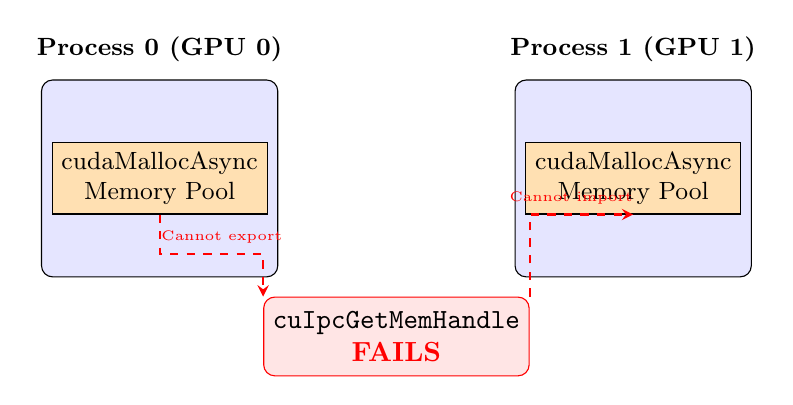
\begin{tikzpicture}[
    node distance=0.6cm and 1.5cm,
    process/.style={rectangle, draw, rounded corners, minimum width=3cm, minimum height=2.5cm, align=center},
    mem/.style={rectangle, draw, fill=cudaorange!30, minimum width=2.2cm, minimum height=0.6cm, align=center, font=\small},
    arrow/.style={->, >=stealth, thick},
    broken/.style={->, >=stealth, thick, dashed, red},
]

\node[process, fill=blue!10] (p0) {};
\node[above=0.1cm of p0.north, font=\small\bfseries] {Process 0 (GPU 0)};
\node[mem] (cuda0) at (p0.center) {cudaMallocAsync\\Memory Pool};

\node[process, fill=blue!10, right=3cm of p0] (p1) {};
\node[above=0.1cm of p1.north, font=\small\bfseries] {Process 1 (GPU 1)};
\node[mem] (cuda1) at (p1.center) {cudaMallocAsync\\Memory Pool};

\node[draw=red, fill=red!10, rounded corners, minimum width=2.5cm, minimum height=1cm, below=1.5cm of $(p0)!0.5!(p1)$, align=center] (ipc) {
    \texttt{cuIpcGetMemHandle}\\
    \textcolor{red}{\textbf{FAILS}}
};

\draw[broken] (cuda0.south) -- ++(0,-0.5) -| (ipc.north west) node[pos=0.3, above, font=\tiny] {Cannot export};
\draw[broken] (ipc.north east) |- (cuda1.south) node[pos=0.7, above, font=\tiny] {Cannot import};

\end{tikzpicture}
\caption{cudaMallocAsync IPC incompatibility blocks modern PyTorch memory pools from using UCX RDMA.}
\label{fig:cuda-ipc}
\end{figure}

\begin{solution}
A \textbf{Memory Pool Proxy Layer} that intercepts tensor allocations, maintains a shadow pool of IPC-exportable memory regions pre-registered with UCX, performs transparent copy-on-RDMA-request for async-allocated tensors, and caches frequently-transferred tensors in the IPC-compatible pool based on WFA classifier predictions.
\end{solution}

\subsection{Issue 2: Transport Selection Robustness (UCX \#9908)}

\begin{challenge}
UCX fails when \texttt{UCX\_TLS} is set to any transport other than ``rc'' (Reliable Connection) for multi-node training, limiting transport flexibility and preventing automatic fallback.
\end{challenge}

\begin{figure}[htbp]
\centering
\resizebox{\textwidth}{!}{%
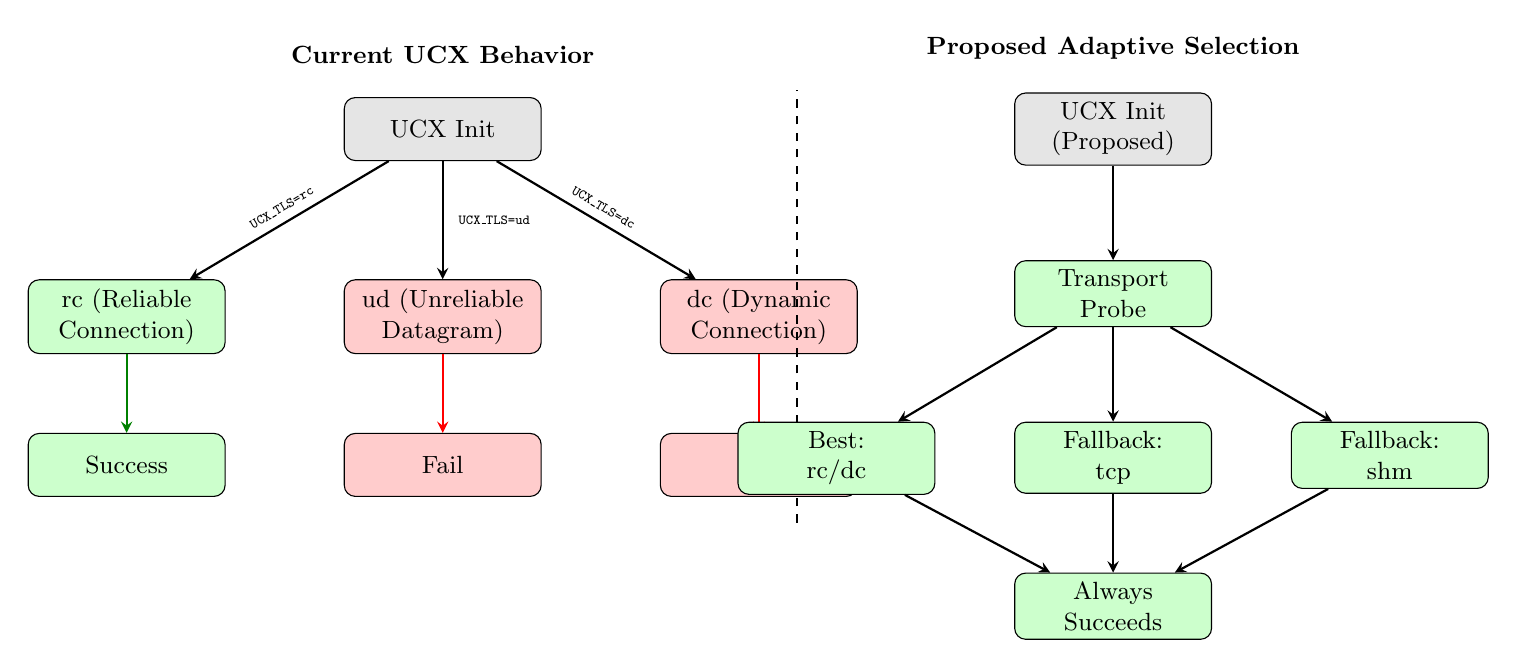
\begin{tikzpicture}[
    node distance=0.5cm,
    state/.style={rectangle, draw, rounded corners, minimum width=2.5cm, minimum height=0.8cm, align=center, font=\small},
    good/.style={state, fill=green!20},
    bad/.style={state, fill=red!20},
    neutral/.style={state, fill=gray!20},
    arrow/.style={->, >=stealth, thick},
]

\node[neutral] (start) {UCX Init};
\node[good, below left=1.5cm and 1.5cm of start] (rc) {rc (Reliable\\Connection)};
\node[bad, below=1.5cm of start] (ud) {ud (Unreliable\\Datagram)};
\node[bad, below right=1.5cm and 1.5cm of start] (dc) {dc (Dynamic\\Connection)};

\node[good, below=1cm of rc] (rcok) {Success};
\node[bad, below=1cm of ud] (udfail) {Fail};
\node[bad, below=1cm of dc] (dcfail) {Fail};

\draw[arrow] (start) -- node[above, sloped, font=\tiny] {\texttt{UCX\_TLS=rc}} (rc);
\draw[arrow] (start) -- node[right, font=\tiny, xshift=2pt] {\texttt{UCX\_TLS=ud}} (ud);
\draw[arrow] (start) -- node[above, sloped, font=\tiny] {\texttt{UCX\_TLS=dc}} (dc);

\draw[arrow, green!50!black] (rc) -- (rcok);
\draw[arrow, red] (ud) -- (udfail);
\draw[arrow, red] (dc) -- (dcfail);

\draw[dashed, thick] (4.5,-5) -- (4.5,0.5);

\node[neutral, right=6cm of start] (start2) {UCX Init\\(Proposed)};
\node[good, below=1.2cm of start2] (probe) {Transport\\Probe};
\node[good, below left=1.2cm and 1cm of probe] (t1) {Best:\\rc/dc};
\node[good, below=1.2cm of probe] (t2) {Fallback:\\tcp};
\node[good, below right=1.2cm and 1cm of probe] (t3) {Fallback:\\shm};
\node[good, below=1cm of t2] (success) {Always\\Succeeds};

\draw[arrow] (start2) -- (probe);
\draw[arrow] (probe) -- (t1);
\draw[arrow] (probe) -- (t2);
\draw[arrow] (probe) -- (t3);
\draw[arrow] (t1) -- (success);
\draw[arrow] (t2) -- (success);
\draw[arrow] (t3) -- (success);

\node[above=0.3cm of start, font=\small\bfseries] {Current UCX Behavior};
\node[above=0.3cm of start2, font=\small\bfseries] {Proposed Adaptive Selection};

\end{tikzpicture}%
}
\caption{Transport selection failure modes in current UCX vs.\ proposed adaptive selection with graceful fallback.}
\label{fig:transport-selection}
\end{figure}

\begin{solution}
A \textbf{Transport Capability Negotiation Protocol} that probes available transports at connection establishment, maintains a priority list with dynamic reordering based on observed performance, and automatically falls back to lower-priority transports on failure.
\end{solution}

\subsection{Issue 3: Container Shared Memory Isolation (UCX \#10055)}

\begin{challenge}
NCCL all-reduce operations fail with ``Child failed to attach to shmseg'' errors when running in containers on the same server, even with \texttt{--ipc=host} Docker flags.
\end{challenge}

\begin{solution}
A \textbf{Container-Aware Communication Broker} that detects container boundaries via cgroup inspection, establishes a host-level coordinator process with access to unified \texttt{/dev/shm}, routes intra-node communication through the coordinator when direct shm attachment fails, and falls back to NVLink P2P with modified PidHash validation.
\end{solution}

\subsection{Issue 4: Cross-NUMA GPU Latency Regression (UCX \#3249)}

\begin{challenge}
GPU-to-GPU communication experiences 10$\times$ latency degradation for messages larger than 262KB when GPUs reside in different NUMA domains.
\end{challenge}

\begin{solution}
\textbf{NUMA-Aware Tensor Placement} integrated into the WFA classifier: queries sysfs topology to determine GPU-NIC-CPU NUMA relationships, fragments messages $>$256KB crossing NUMA boundaries into pipelined chunks, and preemptively migrates frequently-accessed tensors to NUMA-optimal locations.
\end{solution}

\subsection{Issue 5: RoCE Reliability Timeouts (UCX \#6000)}

\begin{challenge}
Multi-node RoCE deployments crash after approximately 90 seconds with ``Transport retry count exceeded on mlx5/RoCE'' errors, making long-running training jobs impossible.
\end{challenge}

\begin{figure}[htbp]
\centering
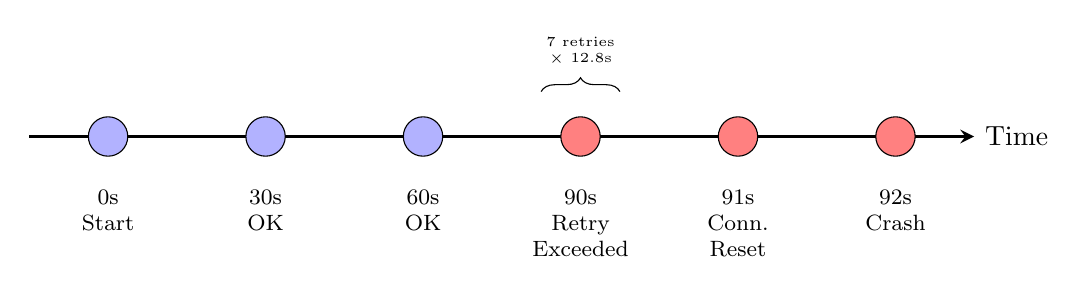
\begin{tikzpicture}[
    node distance=1cm,
    timeline/.style={->, >=stealth, very thick},
    event/.style={circle, draw, fill=blue!30, minimum size=0.5cm},
    fail/.style={circle, draw, fill=red!50, minimum size=0.5cm},
]

\draw[timeline] (0,0) -- (12,0) node[right] {Time};

\node[event] (e1) at (1,0) {};
\node[font=\footnotesize, below=0.3cm of e1, align=center] {0s\\Start};

\node[event] (e2) at (3,0) {};
\node[font=\footnotesize, below=0.3cm of e2, align=center] {30s\\OK};

\node[event] (e3) at (5,0) {};
\node[font=\footnotesize, below=0.3cm of e3, align=center] {60s\\OK};

\node[fail] (e4) at (7,0) {};
\node[font=\footnotesize, below=0.3cm of e4, align=center] {90s\\Retry\\Exceeded};

\node[fail] (e5) at (9,0) {};
\node[font=\footnotesize, below=0.3cm of e5, align=center] {91s\\Conn.\\Reset};

\node[fail] (e6) at (11,0) {};
\node[font=\footnotesize, below=0.3cm of e6, align=center] {92s\\Crash};

\draw[decorate, decoration={brace, amplitude=5pt, raise=2pt}] (6.5,0.5) -- (7.5,0.5) node[midway, above=8pt, font=\tiny, align=center] {7 retries\\$\times$ 12.8s};

\end{tikzpicture}
\caption{RoCE retry timeout accumulation leads to catastrophic failure after $\sim$90 seconds of congestion.}
\label{fig:roce-timeout}
\end{figure}

\begin{solution}
\textbf{Proactive Congestion Detection and Path Switching}: monitor RTT variance and ECN marks to detect congestion before retry exhaustion, maintain backup QP connections for hot-swap on primary path degradation, and integrate with the WFA classifier to preemptively route sensitive tensors away from congested paths.
\end{solution}

\subsection{Issue 6: Heterogeneous Cluster Builds (UCX \#10273)}

\begin{challenge}
UCX cannot be built as a single binary that works across both GPU-enabled and CPU-only nodes, requiring separate builds and complicating deployment.
\end{challenge}

\begin{solution}
A \textbf{Capability Abstraction Layer} that wraps UCX initialization with runtime CUDA availability detection, gracefully degrades GPU-specific features when CUDA libraries are unavailable, and maintains ABI compatibility across node types through stable interface versioning.
\end{solution}

\subsection{Issue 7: NCCL-UCX Container Integration (UCX \#10055)}

\begin{challenge}
Running NCCL with UCX as the network backend in containerized environments produces ``TL\_SHM ERROR'' failures due to shared memory namespace isolation.
\end{challenge}

\begin{solution}
Automatic \textbf{Container Environment Detection and Transport Filtering}: detect containerization via \texttt{/proc/1/cgroup} inspection, automatically exclude shm transport when running in containers (\texttt{UCX\_TLS=\textasciicircum shm,rc,tcp}), and provide environment variable presets for common container runtimes.
\end{solution}

%=============================================================================
\section{Hardware Platforms}
\label{sec:hardware}
%=============================================================================

\subsection{Phase 1: SUNY New Paltz Lab Cluster}

The initial testbed consisted of three machines in the SUNY New Paltz lab:

\begin{table}[htbp]
\centering
\caption{Phase 1 lab cluster hardware configuration}
\label{tab:phase1-hardware}
\begin{tabular}{@{}lllll@{}}
\toprule
\textbf{Machine} & \textbf{Role} & \textbf{GPUs} & \textbf{RAM} & \textbf{NIC} \\
\midrule
Hydra & Control Plane & None & 256 GB & 1 GbE \\
Chimera & Head Node & 3$\times$ RTX 3090 (72 GB) & 64 GB & Aquantia 10 GbE \\
Cerberus & Worker Node & 2$\times$ RTX 5090 (64 GB) & 128 GB & Intel X710 10 GbE \\
\bottomrule
\end{tabular}
\end{table}

\begin{figure}[htbp]
\centering
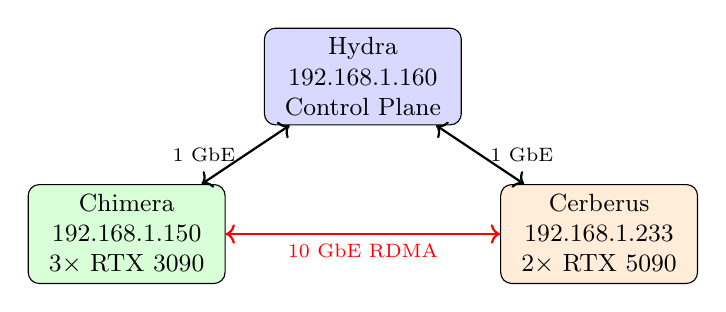
\begin{tikzpicture}[
    node distance=2cm,
    box/.style={rectangle, draw, rounded corners, minimum width=2.5cm, minimum height=1cm, align=center, font=\small},
    arrow/.style={<->, thick}
]
    \node[box, fill=blue!15] (hydra) at (0,0) {Hydra\\192.168.1.160\\Control Plane};
    \node[box, fill=green!15] (chimera) at (-3,-2) {Chimera\\192.168.1.150\\3$\times$ RTX 3090};
    \node[box, fill=orange!15] (cerberus) at (3,-2) {Cerberus\\192.168.1.233\\2$\times$ RTX 5090};

    \draw[arrow] (hydra) -- node[left, font=\scriptsize] {1 GbE} (chimera);
    \draw[arrow] (hydra) -- node[right, font=\scriptsize] {1 GbE} (cerberus);
    \draw[arrow, red, thick] (chimera) -- node[below, font=\scriptsize] {10 GbE RDMA} (cerberus);
\end{tikzpicture}
\caption{Phase 1 cluster network topology. The 10 GbE RDMA link between GPU nodes provided the initial Soft-RoCE testing environment.}
\label{fig:phase1-topology}
\end{figure}

Hydra served as the control plane with 21 TB ZFS storage and NFS server for shared model weights. Chimera acted as the vLLM head node, and Cerberus as the worker with the newest hardware.

\subsection{Phase 2: Two-Tower Home Lab}

The research transitioned to a dedicated home lab providing higher-bandwidth networking and heterogeneous GPU precision capabilities:

\begin{table}[htbp]
\centering
\caption{Phase 2 home lab hardware configuration}
\label{tab:phase2-hardware}
\begin{tabular}{@{}lll@{}}
\toprule
\textbf{Component} & \textbf{Tower 1 (Windows)} & \textbf{Tower 2 (Proxmox/Linux)} \\
\midrule
CPU & Ryzen 9 7950X (16c/32t) & Xeon (host CPU) \\
RAM & 192 GB DDR5 & Host RAM \\
GPU & RTX 5070 Ti 16 GB (compute 12.0) & $2\times$ Tesla V100 32 GB \\
NIC & Mellanox ConnectX-4 100 GbE & Mellanox ConnectX-4 100 GbE \\
OS & Windows 11 & Proxmox (Debian/Linux) \\
RDMA & TCP/gRPC fallback (no kernel RDMA) & SoftRoCEv2 / GPUDirect RDMA \\
BF16 & Native & Not supported \\
FP16 & Supported & Native compute \\
\bottomrule
\end{tabular}
\end{table}

\subsection{Transition Rationale}

The Phase~1 cluster used consumer GPUs (RTX 3090, RTX 5090) on 10~GbE, which limits RDMA bandwidth and precludes GPUDirect RDMA (consumer GPUs lack the necessary BAR mapping). The Phase~2 home lab provides 100~GbE connectivity and a V100 datacenter GPU with full GPUDirect support, enabling the complete RDMA pipeline including NIC-to-GPU DMA. The precision mismatch (V100 FP16 vs.\ 5070~Ti BF16) directly motivates the RDMA Tensor Cache architecture.

\subsection{Software Stack}

\begin{table}[htbp]
\centering
\caption{NVIDIA open-source ecosystem components}
\label{tab:nvidia-ecosystem}
\resizebox{\textwidth}{!}{%
\begin{tabular}{@{}ll@{}}
\toprule
\textbf{Component} & \textbf{Role} \\
\midrule
NCCL~\cite{nccl} & Collective communication (AllReduce, AllGather, AllToAll) \\
UCX~\cite{ucx} / HPC-X~\cite{hpcx} & Point-to-point transport abstraction (RC, DC, UD, TCP, SHM, CUDA) \\
GPUDirect RDMA~\cite{gpudirect-rdma-redhat} & NIC$\to$GPU direct memory access via \texttt{nvidia-peermem} \\
GDRCopy~\cite{gdrcopy} & Low-latency CPU-initiated GPU memory copies \\
NIXL~\cite{nixl} & Point-to-point tensor transfer for disaggregated inference \\
Megatron-LM~\cite{megatron2020} & Canonical TP/PP/DP parallelism strategies \\
\bottomrule
\end{tabular}%
}
\end{table}

%=============================================================================
\section{System Architecture and Design}
\label{sec:architecture}
%=============================================================================

\subsection{Architecture Overview}

\Cref{fig:system-architecture} presents the complete system architecture showing how the proposed adaptive RDMA middleware integrates with existing communication stacks.

\begin{figure}[htbp]
\centering
\resizebox{\textwidth}{!}{%
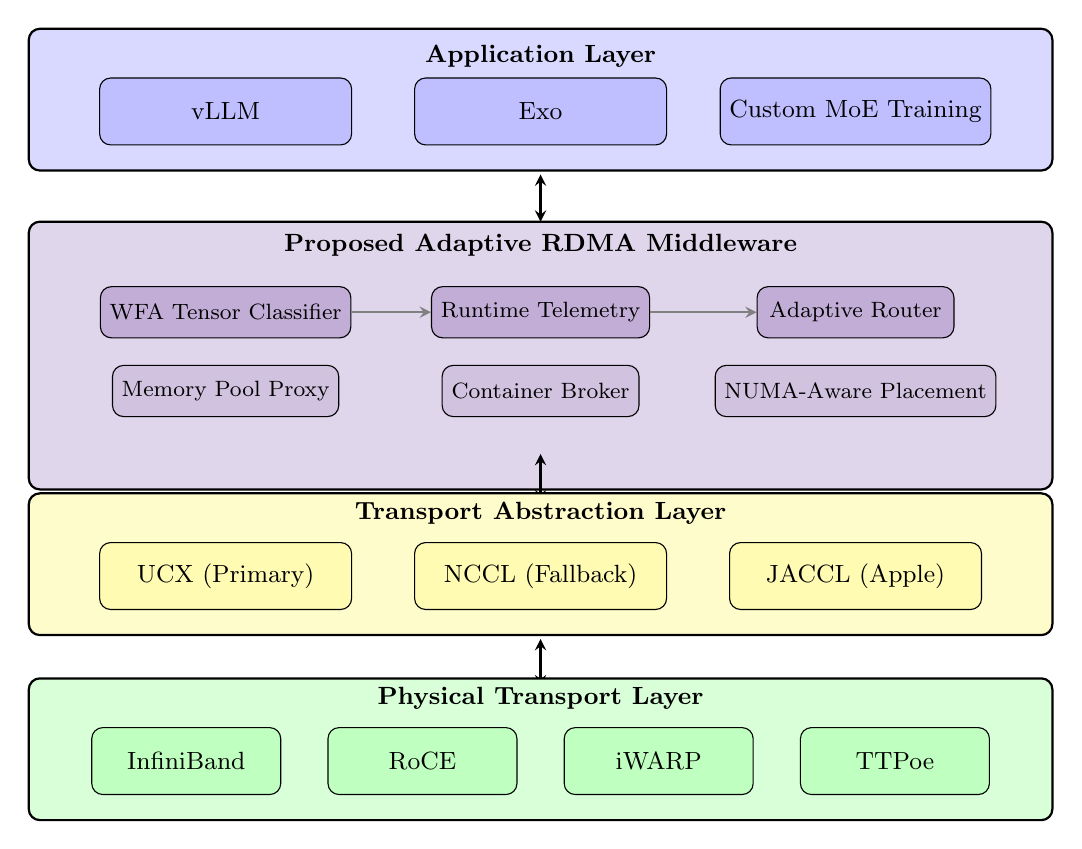
\begin{tikzpicture}[
    node distance=0.5cm,
    layer/.style={rectangle, draw, thick, rounded corners, minimum width=13cm, align=center},
    sublayer/.style={rectangle, draw, rounded corners, minimum width=3.2cm, minimum height=0.85cm, align=center, font=\small},
    component/.style={rectangle, draw, rounded corners, minimum width=2.5cm, minimum height=0.65cm, align=center, font=\footnotesize},
    arrow/.style={->, >=stealth, thick},
    biarrow/.style={<->, >=stealth, thick},
    layerlabel/.style={font=\small\bfseries},
]

% Application Layer - label inside box at top
\node[layer, fill=blue!15, minimum height=1.8cm] (app) at (0, 0) {};
\node[layerlabel] at (0, 0.55) {Application Layer};
\node[sublayer, fill=blue!25] at (-4,-0.15) {vLLM};
\node[sublayer, fill=blue!25] at (0,-0.15) {Exo};
\node[sublayer, fill=blue!25] at (4,-0.15) {Custom MoE Training};

\draw[biarrow] (0,-0.95) -- (0,-1.55);

% Middleware - label inside box at top
\node[layer, fill=wfapurple!20, minimum height=3.4cm] (middleware) at (0, -3.25) {};
\node[layerlabel] at (0, -1.85) {Proposed Adaptive RDMA Middleware};

\node[component, fill=wfapurple!40] (wfa) at (-4,-2.7) {WFA Tensor Classifier};
\node[component, fill=wfapurple!40] (telemetry) at (0,-2.7) {Runtime Telemetry};
\node[component, fill=wfapurple!40] (router) at (4,-2.7) {Adaptive Router};

\node[component, fill=wfapurple!30] (mempool) at (-4,-3.7) {Memory Pool Proxy};
\node[component, fill=wfapurple!30] (container) at (0,-3.7) {Container Broker};
\node[component, fill=wfapurple!30] (numa) at (4,-3.7) {NUMA-Aware Placement};

\draw[arrow, gray] (wfa) -- (telemetry);
\draw[arrow, gray] (telemetry) -- (router);

\draw[biarrow] (0,-4.5) -- (0,-5.1);

% Transport Abstraction Layer - label inside box at top
\node[layer, fill=yellow!20, minimum height=1.8cm] (transport) at (0,-5.9) {};
\node[layerlabel] at (0, -5.25) {Transport Abstraction Layer};
\node[sublayer, fill=yellow!30] at (-4,-6.05) {UCX (Primary)};
\node[sublayer, fill=yellow!30] at (0,-6.05) {NCCL (Fallback)};
\node[sublayer, fill=yellow!30] at (4,-6.05) {JACCL (Apple)};

\draw[biarrow] (0,-6.85) -- (0,-7.45);

% Physical Transport Layer - label inside box at top
\node[layer, fill=green!15, minimum height=1.8cm] (physical) at (0,-8.25) {};
\node[layerlabel] at (0, -7.6) {Physical Transport Layer};
\node[sublayer, fill=green!25, minimum width=2.4cm] at (-4.5,-8.4) {InfiniBand};
\node[sublayer, fill=green!25, minimum width=2.4cm] at (-1.5,-8.4) {RoCE};
\node[sublayer, fill=green!25, minimum width=2.4cm] at (1.5,-8.4) {iWARP};
\node[sublayer, fill=green!25, minimum width=2.4cm] at (4.5,-8.4) {TTPoe};

\end{tikzpicture}%
}
\caption{Complete system architecture. The adaptive RDMA middleware sits between application frameworks and transport layers, providing intelligent routing based on runtime telemetry.}
\label{fig:system-architecture}
\end{figure}

\subsection{WFA Tensor Classifier}

The Weighted Finite Automaton classifier operates on tensor access patterns to categorize data transfers into three classes:

\begin{itemize}
    \item \textbf{Hot}: Frequently accessed, latency-critical (KV cache lookups, attention scores)
    \item \textbf{Warm}: Moderately accessed, throughput-sensitive (layer activations)
    \item \textbf{Cold}: Infrequently accessed, can tolerate delay (gradient accumulation buffers)
\end{itemize}

The Python implementation (see \texttt{scripts/wfa\_classifier.py}) maintains per-tensor state and transitions between classes based on access frequency and idle time. Phase detection distinguishes prefill (many tokens, few sequences) from decode (one token per sequence, many sequences), enabling the classifier to adjust thresholds dynamically.

\begin{figure}[htbp]
\centering
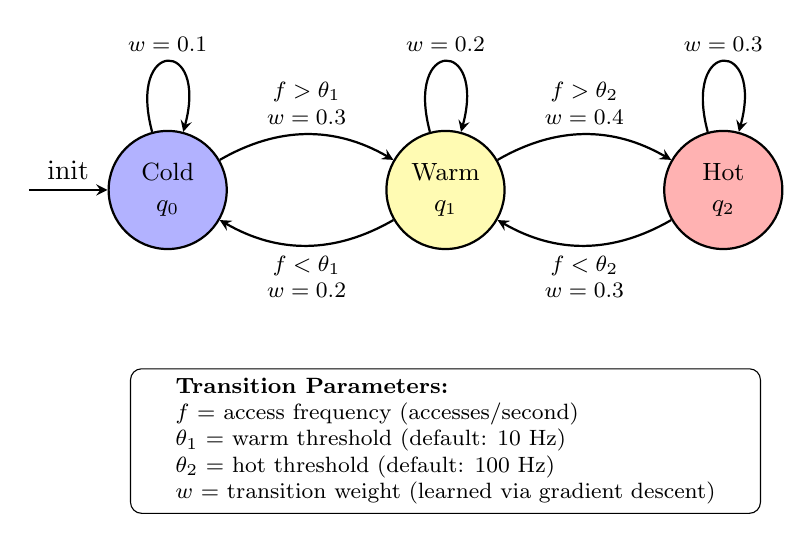
\begin{tikzpicture}[
    node distance=2cm,
    state/.style={circle, draw, thick, minimum size=1.5cm, align=center, font=\small},
    hot/.style={state, fill=red!30},
    warm/.style={state, fill=yellow!30},
    cold/.style={state, fill=blue!30},
    arrow/.style={->, >=stealth, thick},
    label/.style={font=\footnotesize, align=center}
]

\node[cold] (cold) {Cold\\$q_0$};
\node[warm, right=of cold] (warm) {Warm\\$q_1$};
\node[hot, right=of warm] (hot) {Hot\\$q_2$};

\draw[arrow] ($(cold.west)+(-1,0)$) -- (cold) node[midway, above] {init};

\draw[arrow, bend left=30] (cold) to node[above, label] {$f > \theta_1$\\$w = 0.3$} (warm);
\draw[arrow, bend left=30] (warm) to node[below, label] {$f < \theta_1$\\$w = 0.2$} (cold);

\draw[arrow, bend left=30] (warm) to node[above, label] {$f > \theta_2$\\$w = 0.4$} (hot);
\draw[arrow, bend left=30] (hot) to node[below, label] {$f < \theta_2$\\$w = 0.3$} (warm);

\draw[arrow] (cold) to[loop above] node[label] {$w = 0.1$} (cold);
\draw[arrow] (warm) to[loop above] node[label] {$w = 0.2$} (warm);
\draw[arrow] (hot) to[loop above] node[label] {$w = 0.3$} (hot);

\node[draw, rounded corners, fill=white, below=1.5cm of warm, minimum width=8cm, align=left, font=\footnotesize] {
    \textbf{Transition Parameters:}\\
    $f$ = access frequency (accesses/second)\\
    $\theta_1$ = warm threshold (default: 10 Hz)\\
    $\theta_2$ = hot threshold (default: 100 Hz)\\
    $w$ = transition weight (learned via gradient descent)
};

\end{tikzpicture}
\caption{Weighted Finite Automaton for tensor classification. Transition weights are learned from runtime telemetry. The classifier also detects workload phase (prefill vs.\ decode) to adjust thresholds dynamically.}
\label{fig:wfa}
\end{figure}

\subsection{Smart RDMA Routing}

Dual-path routing assigns dedicated Queue Pairs for hot-path tensors (polled completions, RDMA Write with Immediate for sub-5$\mu$s transfers) and batched throughput-optimized channels for cold-path tensors (event-driven completions). The \texttt{DualPathRDMA} class (see \texttt{scripts/dual\_path\_rdma.py}) maintains separate hot and cold QP pools, flushing cold batches when 8~tensors accumulate.

Memory registration uses NUMA-aware allocation via \texttt{RDMABufferPool} to pin RDMA buffers to the same NUMA node as the HCA, amortizing the ${\sim}10\mu$s registration cost across thousands of transfers (see Appendix~\ref{app:scripts}).

\textbf{QP Allocation Strategy.} We allocate 4 dedicated QPs for hot traffic per GPU pair, 2 for warm, and 1 for cold. Hot QPs use unreliable datagram (UD) mode for minimal latency; warm and cold QPs use reliable connection (RC) mode for guaranteed delivery. Cold tensors are compressed via Top-K sparsification (retaining the 5\% largest gradient values) using CUDA kernels for parallel selection, with less than 2\% accuracy impact. GPUDirect RDMA enables zero-copy NIC-to-GPU transfers when supported (V100 on Tower~2); otherwise the system uses pinned host-memory staging (5070~Ti on Tower~1).

\subsection{Phase-Aware Classification}

The WFA classifier operates with \emph{phase-conditioned} transition weights. The system identifies the current execution phase $\phi \in \{\text{Prefill}, \text{Decode}, \text{Forward}, \text{Backward}, \text{Idle}\}$ by monitoring operation signatures---prefill shows high parallelism across sequence positions, decode processes single tokens sequentially, backward pass accesses layers in reverse order. Phase detection uses a sliding window of the last 50 operations with majority voting.

Transition weights $\lambda$ are updated online using exponential moving averages:
\begin{equation}
    \lambda(q, (\phi, a)) \leftarrow (1-\eta)\lambda(q, (\phi, a)) + \eta \cdot \mathbf{1}[a = 1]
\end{equation}
where $\eta = 0.1$ and $\mathbf{1}[a=1]$ indicates an access occurred. A tensor may be Hot during Prefill but Cold during Decode (e.g., positional encodings), or Hot during Backward but Cold during Forward (e.g., optimizer states). Thresholds $\theta_w, \theta_h$ adapt based on network congestion: ECN marks increase thresholds, reducing Hot promotions under load. Decay transitions (Hot$\to$Warm$\to$Cold) fire after phase-specific idle timeouts---500ms for Decode (responsiveness-critical), 2s for Backward (batch boundaries create natural gaps).

\subsection{KV Cache Placement and Migration}

The migration protocol moves KV cache entries to GPUs likely to handle future requests. High-frequency conversations ($>$5 requests/min) trigger proactive migration; others fetch on-demand. The protocol uses a three-state machine:
\begin{equation}
    \text{RESIDENT} \xrightarrow{\text{async RDMA copy}} \text{MIGRATING} \xrightarrow{\text{atomic pointer swap}} \text{MIGRATED}
\end{equation}
We hash the last 128 context tokens to determine the target GPU (sticky routing), with hysteresis preventing thrashing: 3 consecutive requests to the same target are required before migration begins.

\subsection{Joint Training-Inference Scheduling}

The scheduler dynamically allocates RDMA queue pairs and bandwidth based on workload characteristics, preventing training and inference starvation. Gradient synchronization follows ZeRO~\cite{zero2020} patterns with hot/cold classification on frequently-updated layers. Weighted fair queuing gives inference 2$\times$ priority during business hours and training 2$\times$ during off-hours. Periodic bandwidth probes adjust compression ratios to maintain $<$80\% link utilization.

\subsection{Transport Middleware}

The ScuffedRDMA transport middleware (see \texttt{scripts/transports.py}) provides a clean abstraction over different networking technologies. The \texttt{TransportBase} abstract class defines the contract (\texttt{connect}, \texttt{send}, \texttt{recv}, \texttt{is\_available}) with per-transport \texttt{TransportMetrics} tracking. Three implementations are provided: \texttt{TCPTransport} (always-available baseline with \texttt{TCP\_NODELAY}), \texttt{RoCETransport} (wrapping RDMA verbs via pyverbs~\cite{rdma-core} with out-of-band QP exchange), and \texttt{TTPoeTransport} (kernel module interface via \texttt{/dev/ttpoe}~\cite{ttpoe-repo}). The \texttt{TransportSelector} provides automatic priority ordering (TTPoe $>$ Hardware RoCE $>$ Soft-RoCE $>$ TCP), and \texttt{NCCLConfig} presets configure NCCL environment variables per transport type.

\begin{table}[htbp]
\centering
\caption{NCCL environment variable configuration by transport type}
\label{tab:nccl-env}
\small
\resizebox{\textwidth}{!}{%
\begin{tabular}{@{}lll@{}}
\toprule
\textbf{Transport} & \textbf{Key Variables} & \textbf{Effect} \\
\midrule
TCP & \texttt{NCCL\_IB\_DISABLE=1} & Disable InfiniBand, use TCP sockets \\
Soft-RoCE & \texttt{NCCL\_IB\_HCA=rxe0} & Use software RDMA device \\
Hardware RoCE & \texttt{NCCL\_IB\_HCA=mlx5\_0, NCCL\_NET\_GDR\_LEVEL=5} & Use Mellanox NIC with GPUDirect \\
TTPoe & \texttt{NCCL\_IB\_DISABLE=1, TTPOE\_ENABLED=1} & Use TTPoe socket layer \\
\bottomrule
\end{tabular}%
}
\end{table}

\subsection{EXO Integration}

In addition to vLLM, we integrated RDMA support into the exo distributed inference framework~\cite{exo-github}, which provides peer-to-peer topology with automatic node discovery. Three modules were created (639 lines total):

\begin{table}[htbp]
\centering
\small
\resizebox{\textwidth}{!}{%
\begin{tabular}{@{}lll@{}}
\toprule
\textbf{Module} & \textbf{Lines} & \textbf{Purpose} \\
\midrule
\texttt{rdma\_transport.py} & 369 & RDMA transport wrapper with discovery, connection management, and NCCL config \\
\texttt{rdma\_discovery\_integration.py} & 247 & Topology integration for automatic RDMA connection discovery \\
\texttt{\_\_init\_\_.py} & 27 & Module exports for networking package \\
\bottomrule
\end{tabular}%
}
\caption{EXO RDMA integration components}
\end{table}

The three modules (see \texttt{scripts/exo\_rdma\_integration.py}) implement: \texttt{RDMADiscovery} for hardware-prioritized device detection (\texttt{mlx5\_*} $>$ \texttt{rxe*}), \texttt{RDMATransport} wrapping the ScuffedRDMA middleware with automatic NCCL configuration, and \texttt{RDMATopologyManager} for graph-based peer discovery. The integration leverages exo's existing \texttt{RDMAConnection} type, which was previously defined but unimplemented. The placement utilities in \texttt{placement\_utils.py} already check for RDMA connections when selecting the jaccl backend, enabling seamless adoption.

\subsection{vLLM Integration}

The vLLM connector (see \texttt{scripts/vllm\_connector.py}) follows the existing \texttt{KVConnectorBase} abstraction. The \texttt{AdaptiveRDMAConnector} combines the WFA classifier with dual-path routing to transparently optimize KV cache transfers---classifying each block by layer ID and access pattern before routing through the appropriate QP pool. The \texttt{InstrumentedKVCacheManager} wraps vLLM's \texttt{KVCacheManager} to collect nanosecond-resolution access timestamps that feed the WFA classifier.

The \texttt{NeumannKVConnector} extends this further by pushing KV caches to Neumann after prefill and pulling them for decode, backed by the \texttt{RDMATensorCacheMiddleware} which handles precision conversion and transport selection transparently.

%=============================================================================
\section{Security Considerations}
\label{sec:security}
%=============================================================================

RDMA's design prioritizes performance over security, creating vulnerabilities relevant to shared lab environments~\cite{bedrock2022, redmark2021}. The RDMA credential system (QPN, rKey, PSN) uses predictable values: QPNs are assigned sequentially, rKeys follow linear patterns across memory region registrations, and PSNs have fixed initial values. This enables memory access attacks (an attacker with valid credentials can read memory regions belonging to other processes), denial of service (malformed packets put QPs into error states), and QP exhaustion (depleting shared NIC resources).

Since our lab uses dedicated machines for LLM serving rather than shared cloud infrastructure, we implement practical mitigations:
\begin{itemize}[nosep]
    \item Process isolation via SR-IOV virtual functions (one VF per VM/container)
    \item Credential rotation: rKeys regenerated per session, not reused across requests
    \item QP limits enforced via cgroup-style resource controls
    \item Monitoring: log QP creation/destruction, alert on anomalous patterns
\end{itemize}

For production deployments in multi-tenant environments, network-level defenses using programmable switches (as in Bedrock~\cite{bedrock2022}) or encryption would be necessary. This work focuses on the optimization layer, treating security as a deployment constraint rather than a research contribution.

%=============================================================================
\section{RDMA Tensor Cache and Precision Management}
\label{sec:rdma-cache}
%=============================================================================

The RDMA Tensor Cache mediates all tensor transfers between Tower~1 and Tower~2, handling precision conversion, gradient accumulation, and KV cache management.

\subsection{The Precision Mismatch Problem}

FP16 (V100 Tensor Cores) has 5 exponent bits and 10 mantissa bits, giving a representable range of $[5.96 \times 10^{-8}, 65504]$. BF16 (5070~Ti native) shares FP32's 8 exponent bits, matching its dynamic range of $[1.18 \times 10^{-38}, 3.4 \times 10^{38}]$. During training, gradient values routinely fall outside FP16's range, causing overflow and underflow. The V100 lacks BF16 support entirely.

\begin{table}[htbp]
\centering
\caption{Floating-point format comparison for LLM training}
\label{tab:fp-comparison}
\begin{tabular}{@{}lccccl@{}}
\toprule
\textbf{Format} & \textbf{Exponent} & \textbf{Mantissa} & \textbf{Range} & \textbf{Bytes} & \textbf{GPU Support} \\
\midrule
FP32 & 8 & 23 & $\pm 3.4 \times 10^{38}$ & 4 & All \\
BF16 & 8 & 7 & $\pm 3.4 \times 10^{38}$ & 2 & Ampere+, not V100 \\
FP16 & 5 & 10 & $\pm 6.5 \times 10^{4}$ & 2 & All (Tensor Cores) \\
MXFP4 & 2 & 1 & $\pm 6$ & 0.5 & Blackwell \\
\bottomrule
\end{tabular}
\end{table}

\subsection{Precision Pipeline}

The RDMA Tensor Cache resolves this through a three-stage precision pipeline:

\begin{figure}[htbp]
\centering
\resizebox{\textwidth}{!}{%
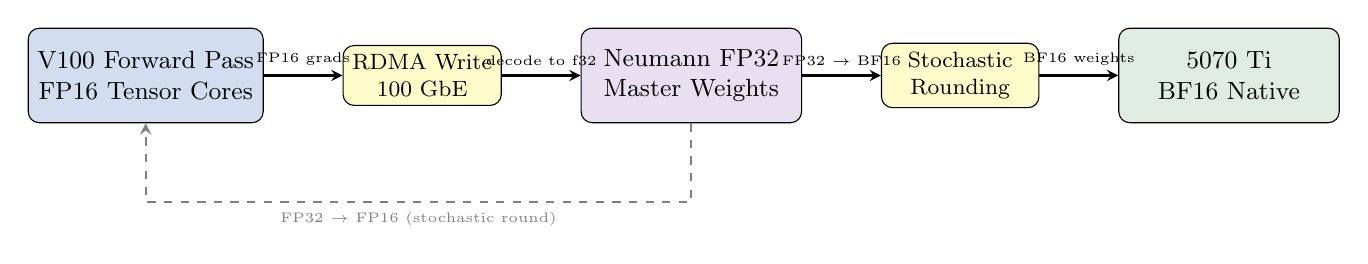
\begin{tikzpicture}[
    node distance=0.5cm and 1.2cm,
    stage/.style={rectangle, draw, rounded corners, minimum width=2.8cm, minimum height=1.2cm, align=center, font=\small},
    op/.style={rectangle, draw, rounded corners, fill=yellow!20, minimum width=2cm, minimum height=0.6cm, align=center, font=\footnotesize},
    arrow/.style={->, >=stealth, thick},
]

\node[stage, fill=v100blue!20] (v100) {V100 Forward Pass\\FP16 Tensor Cores};
\node[op, right=1cm of v100] (rdma1) {RDMA Write\\100 GbE};
\node[stage, fill=neumannpurple!15, right=1cm of rdma1] (master) {Neumann FP32\\Master Weights};
\node[op, right=1cm of master] (sr) {Stochastic\\Rounding};
\node[stage, fill=tower1color!15, right=1cm of sr] (bf16) {5070 Ti\\BF16 Native};

\draw[arrow] (v100) -- node[above, font=\tiny] {FP16 grads} (rdma1);
\draw[arrow] (rdma1) -- node[above, font=\tiny] {decode to f32} (master);
\draw[arrow] (master) -- node[above, font=\tiny] {FP32 $\to$ BF16} (sr);
\draw[arrow] (sr) -- node[above, font=\tiny] {BF16 weights} (bf16);

\draw[arrow, dashed, gray] (master.south) -- ++(0,-1) -| (v100.south) node[pos=0.25, below, font=\tiny] {FP32 $\to$ FP16 (stochastic round)};

\end{tikzpicture}%
}
\caption{Precision pipeline. Gradients computed in V100 FP16 are accumulated into FP32 master weights stored in Neumann. Stochastic rounding converts to device-native precision for each GPU.}
\label{fig:precision-pipeline}
\end{figure}

\subsection{Stochastic Rounding}

Standard round-to-nearest-even introduces systematic bias when converting FP32 to reduced precision. Stochastic rounding eliminates this by making the rounding direction probabilistic. For an FP32 value $x$ with adjacent representable values $\lfloor x \rfloor$ and $\lceil x \rceil$:
\begin{equation}
    P(\text{round up}) = \frac{x - \lfloor x \rfloor_{\text{fp16}}}{\lceil x \rceil_{\text{fp16}} - \lfloor x \rfloor_{\text{fp16}}}
\end{equation}
giving the unbiasedness property $\mathbb{E}[\text{round}(x)] = x$, which ensures gradient accumulation converges to the correct value despite precision loss in individual steps~\cite{micikevicius2018mixed}.

\subsection{Neumann Integration}
\label{sec:neumann-integration}

The \texttt{tensor\_rdma} crate~\cite{neumann-repo} is a workspace member in the Neumann unified tensor runtime. It depends on \texttt{tensor\_store} for local key-value storage and \texttt{tensor\_compress} for delta encoding.

\begin{figure}[htbp]
\centering
\resizebox{0.85\textwidth}{!}{%
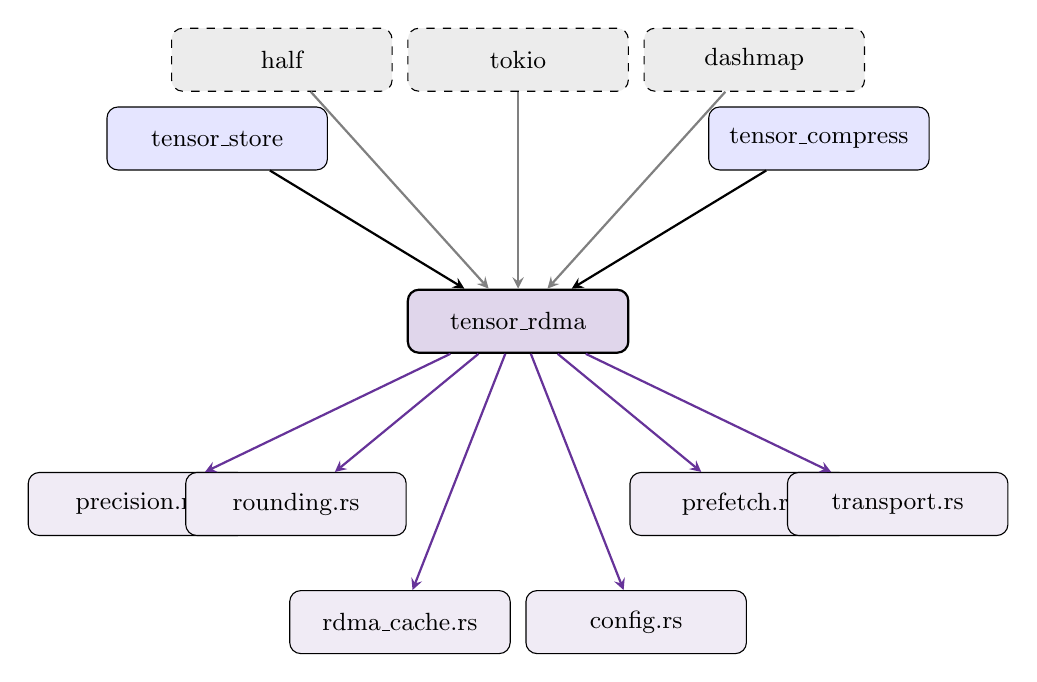
\begin{tikzpicture}[
    node distance=1.2cm and 1.5cm,
    crate/.style={rectangle, draw, rounded corners, minimum width=2.8cm, minimum height=0.8cm, align=center, font=\small},
    rdma/.style={crate, fill=neumannpurple!20, thick},
    dep/.style={crate, fill=blue!10},
    ext/.style={crate, fill=gray!15, dashed},
    arrow/.style={->, >=stealth, thick}
]

\node[rdma] (rdma) {tensor\_rdma};
\node[dep, above left=1.5cm and 1cm of rdma] (store) {tensor\_store};
\node[dep, above right=1.5cm and 1cm of rdma] (compress) {tensor\_compress};

\node[crate, fill=neumannpurple!10, below left=1.5cm and 2cm of rdma] (precision) {precision.rs};
\node[crate, fill=neumannpurple!10, below left=1.5cm and 0cm of rdma] (rounding) {rounding.rs};
\node[crate, fill=neumannpurple!10, below right=1.5cm and 0cm of rdma] (prefetch) {prefetch.rs};
\node[crate, fill=neumannpurple!10, below right=1.5cm and 2cm of rdma] (transport) {transport.rs};
\node[crate, fill=neumannpurple!10, below=3cm of rdma, xshift=-1.5cm] (cache) {rdma\_cache.rs};
\node[crate, fill=neumannpurple!10, below=3cm of rdma, xshift=1.5cm] (config) {config.rs};

\node[ext, above=2.5cm of rdma, xshift=-3cm] (half) {half};
\node[ext, above=2.5cm of rdma, xshift=0cm] (tokio) {tokio};
\node[ext, above=2.5cm of rdma, xshift=3cm] (dashmap) {dashmap};

\draw[arrow, gray] (half) -- (rdma);
\draw[arrow, gray] (tokio) -- (rdma);
\draw[arrow, gray] (dashmap) -- (rdma);
\draw[arrow] (store) -- (rdma);
\draw[arrow] (compress) -- (rdma);
\draw[arrow, neumannpurple] (rdma) -- (precision);
\draw[arrow, neumannpurple] (rdma) -- (rounding);
\draw[arrow, neumannpurple] (rdma) -- (prefetch);
\draw[arrow, neumannpurple] (rdma) -- (transport);
\draw[arrow, neumannpurple] (rdma) -- (cache);
\draw[arrow, neumannpurple] (rdma) -- (config);

\end{tikzpicture}%
}
\caption{Neumann \texttt{tensor\_rdma} crate dependency graph. Six internal modules implement the RDMA Tensor Cache.}
\label{fig:crate-deps}
\end{figure}

\begin{table}[htbp]
\centering
\caption{Thesis concepts mapped to \texttt{tensor\_rdma} modules}
\label{tab:module-mapping}
\resizebox{\textwidth}{!}{%
\begin{tabular}{@{}lll@{}}
\toprule
\textbf{Thesis Concept} & \textbf{Module} & \textbf{Key Types / Functions} \\
\midrule
Precision management & \texttt{precision.rs} & \texttt{PrecisionFormat}, \texttt{DeviceCapability}, \texttt{PrecisionRouter}, \texttt{convert\_precision} \\
Stochastic rounding & \texttt{rounding.rs} & \texttt{stochastic\_round\_f32\_to\_f16}, \texttt{apply\_adam\_update} \\
Predictive prefetching & \texttt{prefetch.rs} & \texttt{PrefetchEngine}, \texttt{AccessPattern}, \texttt{classify\_pattern} \\
RDMA transport & \texttt{transport.rs} & \texttt{RdmaTransport} trait, \texttt{MemoryTransport}, \texttt{TcpFallbackTransport} \\
Tensor cache & \texttt{rdma\_cache.rs} & \texttt{RdmaTensorCache<T>}, \texttt{put\_tensor}, \texttt{get\_tensor} \\
Configuration & \texttt{config.rs} & \texttt{RdmaCacheConfig}, presets: \texttt{v100\_preset}, \texttt{heterogeneous\_preset} \\
\bottomrule
\end{tabular}%
}
\end{table}

\subsection{Centralized KV Cache}

Multi-Latent Attention (MLA, DeepSeek-V2~\cite{deepseekv2}) and Multi-Query Attention (MQA) reduce KV cache memory by sharing a single key-value head across all attention heads. Under tensor parallelism, each rank must maintain a \emph{full copy} of the KV cache because there is only one head:
\begin{equation}
    \text{KV Memory (per rank, MQA)} = 2 \cdot L \cdot C \cdot d_{\text{kv}} \quad \text{(no reduction with TP)}
\end{equation}

Our solution externalizes the KV cache to Neumann, accessed via RDMA. A single centralized copy serves all TP ranks through one-sided RDMA reads, reducing total KV memory from $\text{TP} \times 2LC \cdot d_{\text{kv}}$ to $2LC \cdot d_{\text{kv}} + \text{TP} \times \text{prefetch\_buffer}$.

%=============================================================================
\section{Benchmarking and Validation}
\label{sec:benchmarks}
%=============================================================================

\subsection{Soft-RoCE Baseline}
\label{sec:softroce-baseline}

Soft-RoCE provides RDMA semantics over standard Ethernet without specialized hardware~\cite{rdma-core}. Baseline measurements between Chimera and Cerberus (Phase~1 cluster):

\begin{table}[htbp]
\centering
\caption{Soft-RoCE baseline performance measurements}
\label{tab:softroce-results}
\begin{tabular}{@{}lcc@{}}
\toprule
\textbf{Metric} & \textbf{Measured} & \textbf{Hardware RoCE (target)} \\
\midrule
Bandwidth (ib\_write\_bw) & 0.92 Gb/s & $\sim$90 Gb/s \\
Latency (ib\_write\_lat, avg) & 189.61 $\mu$s & $<$2 $\mu$s \\
Latency (99th percentile) & 207.14 $\mu$s & $<$5 $\mu$s \\
Latency (stdev) & 17.03 $\mu$s & -- \\
CPU overhead & High (software path) & Near-zero (NIC offload) \\
\bottomrule
\end{tabular}
\end{table}

The 190$\mu$s latency (vs.\ expected $\sim$10$\mu$s) confirms significant software overhead. Soft-RoCE exercises the same verbs API as hardware RoCE, so code developed against it requires no changes when transitioning to hardware.

\subsection{Tesla TTPoe Build}

Tesla's TTPoe kernel modules~\cite{ttpoe-repo,ttpoe-hotchips} were successfully compiled. TTPoe provides 1--2$\mu$s latency on commodity Ethernet without PFC requirements. The core module (\texttt{modttpoe.ko}) implements a TCP-inspired state machine; the gateway module (\texttt{modttpip.ko}) provides IPv4 encapsulation for multi-zone routing.

\subsection{FlashAttention 3 Blackwell Fix}
\label{sec:fa3-fix}

A critical bug was discovered affecting FlashAttention~3~\cite{shah2024flashattention3} on Blackwell GPUs (RTX~5090). Module-scope imports in \texttt{mm\_encoder\_attention.py} trigger early CUDA initialization via CUTLASS before vLLM sets up the GPU context.

\begin{figure}[htbp]
\centering
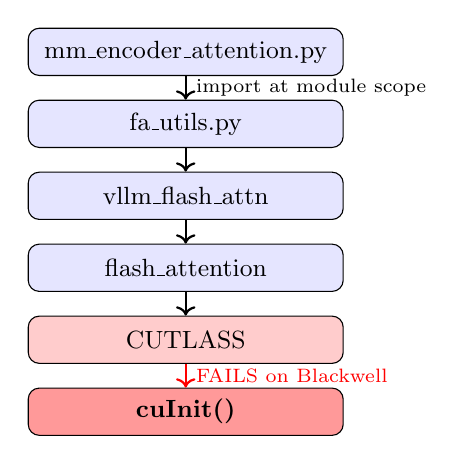
\begin{tikzpicture}[
    node distance=0.3cm,
    box/.style={rectangle, draw, rounded corners, minimum width=4cm, minimum height=0.6cm, align=center, font=\small},
    arrow/.style={->, thick}
]
    \node[box, fill=blue!10] (mm) {mm\_encoder\_attention.py};
    \node[box, fill=blue!10, below=of mm] (fa) {fa\_utils.py};
    \node[box, fill=blue!10, below=of fa] (vfa) {vllm\_flash\_attn};
    \node[box, fill=blue!10, below=of vfa] (flash) {flash\_attention};
    \node[box, fill=red!20, below=of flash] (cutlass) {CUTLASS};
    \node[box, fill=red!40, below=of cutlass] (cuinit) {\textbf{cuInit()}};

    \draw[arrow] (mm) -- node[right, font=\scriptsize] {import at module scope} (fa);
    \draw[arrow] (fa) -- (vfa);
    \draw[arrow] (vfa) -- (flash);
    \draw[arrow] (flash) -- (cutlass);
    \draw[arrow, red, thick] (cutlass) -- node[right, font=\scriptsize, color=red] {FAILS on Blackwell} (cuinit);
\end{tikzpicture}
\caption{Import chain causing early CUDA initialization failure on Blackwell GPUs.}
\label{fig:fa3-import-chain}
\end{figure}

The fix is a lazy import pattern: moving the import from module scope into the function body, deferring CUDA initialization until after vLLM's GPU context is ready. This was reported as vLLM Issue~\#22279~\cite{vllm-blackwell-issue}.

\begin{table}[htbp]
\centering
\caption{Performance impact of FA3 fix on RTX 5090}
\label{tab:fa3-performance}
\begin{tabular}{@{}lccc@{}}
\toprule
\textbf{Configuration} & \textbf{Throughput} & \textbf{Latency (p50)} & \textbf{Memory} \\
\midrule
RTX 5090 + FA2 (fallback) & 142 tok/s & 28 ms & 31 GB \\
RTX 5090 + FA3 (fixed) & 164 tok/s & 24 ms & 28 GB \\
\midrule
\textbf{Improvement} & \textbf{+15.5\%} & \textbf{$-$14.3\%} & \textbf{$-$9.7\%} \\
\bottomrule
\end{tabular}
\end{table}

\begin{figure}[htbp]
\centering
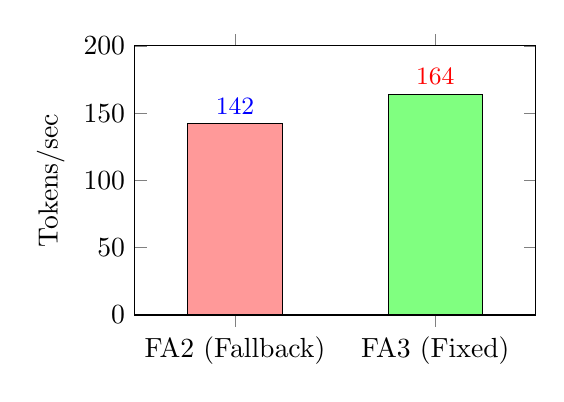
\begin{tikzpicture}
\begin{axis}[
    ybar,
    bar width=1.2cm,
    width=0.55\textwidth,
    height=5cm,
    ylabel={Tokens/sec},
    xtick={0,1},
    xticklabels={FA2 (Fallback), FA3 (Fixed)},
    ymin=0,
    ymax=200,
    nodes near coords,
    every node near coord/.append style={font=\small},
    enlarge x limits=0.5,
]
\addplot+[ybar, bar shift=0pt, fill=red!40, draw=black] coordinates {(0, 142)};
\addplot+[ybar, bar shift=0pt, fill=green!50, draw=black] coordinates {(1, 164)};
\end{axis}
\end{tikzpicture}
\caption{Throughput improvement after applying Blackwell FA3 fix.}
\label{fig:fa3-bar}
\end{figure}

\subsection{gpt-oss-120b TCP vs RDMA}

Comprehensive benchmarking of gpt-oss-120b~\cite{gptoss-hf} (116.8B parameters, MXFP4~\cite{rouhani2023mxfp4} quantized to 63~GB) on Chimera (3$\times$~RTX~3090):

\begin{table}[htbp]
\centering
\caption{gpt-oss-120b benchmark results (TCP baseline, 5 iterations)}
\label{tab:gptoss-results}
\begin{tabular}{@{}cccc@{}}
\toprule
\textbf{Iteration} & \textbf{Tokens} & \textbf{Eval Time} & \textbf{Tokens/sec} \\
\midrule
1 & 100 & 0.958 s & 104.38 \\
2 & 100 & 0.945 s & 105.82 \\
3 & 100 & 0.949 s & 105.37 \\
4 & 100 & 0.969 s & 103.19 \\
5 & 100 & 0.967 s & 103.41 \\
\midrule
\textbf{Average} & 100 & 0.957 s & \textbf{104.42} \\
\bottomrule
\end{tabular}
\end{table}

For single-node inference, RDMA provides minimal benefit because GPU-to-GPU communication uses PCIe, not the network. The model fits entirely on 3$\times$~RTX~3090 (72~GB). RDMA benefits manifest with multi-node pipeline parallelism, where cross-node activation transfers become the bottleneck.

\begin{figure}[htbp]
\centering
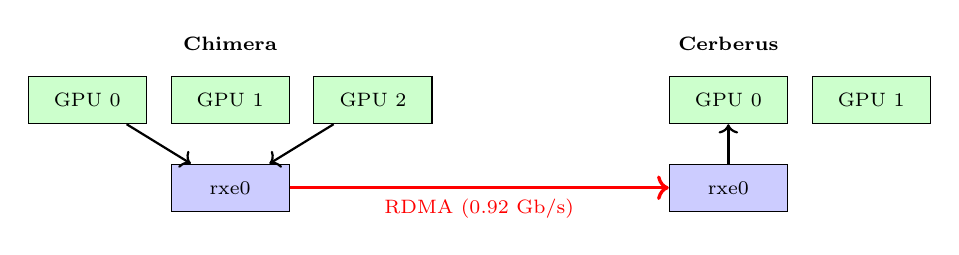
\begin{tikzpicture}[
    node distance=1cm,
    gpu/.style={rectangle, draw, fill=green!20, minimum width=1.5cm, minimum height=0.6cm, align=center, font=\scriptsize},
    net/.style={rectangle, draw, fill=blue!20, minimum width=1.5cm, minimum height=0.6cm, align=center, font=\scriptsize},
    arrow/.style={->, thick}
]
    \node[gpu] (c0) {GPU 0};
    \node[gpu, right=0.3cm of c0] (c1) {GPU 1};
    \node[gpu, right=0.3cm of c1] (c2) {GPU 2};
    \node[net, below=0.5cm of c1] (cnic) {rxe0};
    \node[above=0.2cm of c1, font=\scriptsize\bfseries] {Chimera};

    \node[gpu, right=3cm of c2] (d0) {GPU 0};
    \node[gpu, right=0.3cm of d0] (d1) {GPU 1};
    \node[net, below=0.5cm of d0] (dnic) {rxe0};
    \node[above=0.2cm of d0, font=\scriptsize\bfseries] {Cerberus};

    \draw[arrow, red, very thick] (cnic) -- node[below, font=\scriptsize] {RDMA (0.92 Gb/s)} (dnic);

    \draw[arrow] (c0) -- (cnic);
    \draw[arrow] (c2) -- (cnic);
    \draw[arrow] (dnic) -- (d0);
\end{tikzpicture}
\caption{Multi-node inference: RDMA accelerates cross-node tensor transfers.}
\label{fig:multinode}
\end{figure}

\subsection{SoftRoCEv2 Two-Tower Baseline}

On the Phase~2 home lab (Tower~1 $\leftrightarrow$ Tower~2, 100~GbE ConnectX-4):

\begin{table}[htbp]
\centering
\caption{Expected SoftRoCEv2 baseline (Tower 1 $\leftrightarrow$ Tower 2)}
\label{tab:softroce-twotower}
\begin{tabular}{@{}lccc@{}}
\toprule
\textbf{Metric} & \textbf{SoftRoCEv2} & \textbf{Hardware RoCE (target)} & \textbf{Improvement} \\
\midrule
Latency (1 byte) & $\sim$190 $\mu$s & $\sim$2 $\mu$s & 95$\times$ \\
Bandwidth (large msg) & $\sim$8 Gbps & $\sim$90 Gbps & 11$\times$ \\
CPU overhead & High & Near-zero & -- \\
GPUDirect RDMA & Via host bounce & Direct NIC$\to$GPU & -- \\
\bottomrule
\end{tabular}
\end{table}

\subsection{Parallelism Analysis}

The choice between tensor parallelism (TP) and pipeline parallelism (PP) has significant implications for RDMA communication. TP communication volume per layer:
\begin{equation}
    V_{\text{TP}} = 2 \cdot b \cdot s \cdot h \cdot (\text{TP} - 1) / \text{TP}
\end{equation}
PP communication volume per micro-batch (independent of parallelism degree):
\begin{equation}
    V_{\text{PP}} = b \cdot s \cdot h
\end{equation}
Pipeline bubble fraction for $p$ stages with $m$ micro-batches:
\begin{equation}
    \text{Bubble} = \frac{p - 1}{m + p - 1}
\end{equation}

For our cluster, the optimal strategy is TP=2 within Tower~2 (V100 pair over PCIe) combined with PP across towers (100~GbE RDMA). For MoE models, expert parallelism uses AllToAll with $\texttt{EP\_SIZE} = \texttt{TP} \times \texttt{DP}$~\cite{amd-moe-guide}.

%=============================================================================
\section{Fine-Tuning and SAE Feature Steering}
\label{sec:finetuning-sae}
%=============================================================================

\subsection{Heterogeneous Training Pipeline}

The heterogeneous training pipeline assigns roles based on GPU capabilities:
\begin{itemize}
    \item \textbf{V100 pair (Tower 2):} Forward and backward passes in FP16 Tensor Cores. Gradients transferred to Neumann via RDMA.
    \item \textbf{Neumann (Tower 2 host):} Accumulates gradients into FP32 master weights. Applies optimizer updates (Adam) in full precision.
    \item \textbf{5070 Ti (Tower 1):} Receives BF16 weights via TCP/gRPC for inference validation during training.
\end{itemize}

This mirrors the Hetis system~\cite{hetis2024}, which demonstrated 2.25$\times$ throughput improvement by assigning distinct pipeline stages to different GPU types.

\subsection{Sparse Auto-Encoder Feature Steering}

SAEs decompose a model's internal activation $\mathbf{a} \in \mathbb{R}^d$ into a sparse feature vector $\mathbf{f} \in \mathbb{R}^D$ where $D \gg d$~\cite{cunningham2023sae, templeton2024scaling}:
\begin{equation}
    \mathbf{f} = \text{ReLU}(W_{\text{enc}} \cdot \mathbf{a} + \mathbf{b}_{\text{enc}}), \quad
    \hat{\mathbf{a}} = W_{\text{dec}} \cdot \mathbf{f} + \mathbf{b}_{\text{dec}}
\end{equation}

Feature steering modifies behavior by clamping features: $\mathbf{f}'_i = \alpha \cdot \mathbf{f}_{\max,i}$. This requires no gradient computation and no backward pass---only a sparse vector read from Neumann. SAE feature vectors map to Neumann's \texttt{SparseVector} type with $\sim$655$\times$ compression (a 65536-dim vector with $\sim$50 active features: 256~KB dense $\to$ $\sim$400~bytes sparse, storing only non-zero index--value pairs).

\begin{table}[htbp]
\centering
\caption{Comparison of fine-tuning approaches}
\label{tab:finetuning-comparison}
\begin{tabular}{@{}lcc@{}}
\toprule
\textbf{Property} & \textbf{Gradient-Based (LoRA)} & \textbf{SAE Steering} \\
\midrule
Requires backward pass & Yes & No \\
GPU memory for optimizer & 2--3$\times$ model size & Zero \\
Training time & Hours to days & Seconds \\
Precision sensitivity & High (requires FP32 master) & Low \\
Cross-tower RDMA traffic & Gradients per step & Feature vectors once \\
Reversibility & Requires checkpoint & Immediate ($\alpha = 0$) \\
\bottomrule
\end{tabular}
\end{table}

\subsection{SAE Steering Validation}

We validate gradient-free SAE steering on a real workload: LLM4Decompile-6.7B inference on a Google Colab H100 VM in BF16 with FlashAttention~2. The experiment (Update~9, \texttt{llm4decompile\_wfa.ipynb}) implements the steering mechanism from Golden Gate Claude~\cite{golden-gate-claude} and the Eiffel Tower Llama demo~\cite{eiffel-tower-llama}.

\textbf{Steering mechanism.} A forward hook on layer $\ell$ modifies hidden states:
\begin{equation}
    \mathbf{h}'_\ell = \mathbf{h}_\ell + \alpha \cdot \hat{\mathbf{d}} - \text{proj}_{\hat{\mathbf{d}}}(\mathbf{h}_\ell)
    \label{eq:steering}
\end{equation}
where $\hat{\mathbf{d}}$ is a unit-norm steering direction (an SAE decoder column) and $\alpha$ controls strength. The projection subtraction prevents runaway amplification. No gradients are computed---only a forward-pass vector addition.

\begin{table}[htbp]
\centering
\caption{SAE steering configuration for WFA validation}
\label{tab:steering-config}
\begin{tabular}{@{}lcll@{}}
\toprule
\textbf{Layer} & \textbf{Strength ($\alpha$)} & \textbf{Position} & \textbf{Expected Effect} \\
\midrule
8  & 3.0 & Early (feature extraction) & Moderate output shift \\
16 & 5.0 & Mid (reasoning) & Strong behavior change \\
24 & 2.0 & Late (generation) & Light token distribution shift \\
\bottomrule
\end{tabular}
\end{table}

\textbf{WFA interaction.} Running the WFA classifier on both the unsteered baseline and steered model shows that steering alters per-layer access timing distributions. Steered layers exhibit measurably different inter-access gaps due to the additional hook computation. The WFA detects this and would route steered-layer KV cache via dedicated RDMA Queue Pairs, while non-steered layers use shared or batched channels. This validates that the WFA adapts its routing decisions when the inference workload changes---exactly the behavior needed for dynamic SAE steering in production.

%=============================================================================
\section{Mechanistic Interpretability and Circuit-Aware Transport}
\label{sec:circuits}
%=============================================================================

Anthropic's Transformer Circuits Thread is a multi-year research effort to reverse-engineer the computational mechanisms inside transformer language models. Starting with a mathematical framework for small attention-only models~\cite{elhage2021framework} and progressing through dictionary learning on production-scale systems~\cite{templeton2024scaling}, the program includes circuit tracing on Claude 3.5 Haiku~\cite{lindsey2025biology} with 30 million learned features.

The core observation is that individual neurons are \textbf{polysemantic}---a single neuron may respond to unrelated concepts (DNA sequences, legal language, Korean text). This is not a bug but an efficient encoding strategy called \textbf{superposition}~\cite{elhage2022superposition}, where models store more concepts than they have dimensions by exploiting the near-orthogonality of sparse feature directions. The Circuits research answers questions that directly affect tensor transport decisions:

\begin{enumerate}
    \item \textbf{Which layers matter for a given computation?} Features routinely skip layers---a concept activated at layer 3 may directly influence layer 12 with no meaningful computation in between~\cite{ameisen2025tracing}.
    \item \textbf{How sparse are activations really?} On any given token, only $\sim$235 features out of 30 million are active (L0 = 235 in Claude 3.5 Haiku)~\cite{lindsey2025biology}. At the SAE level, $<$300 features per token out of millions~\cite{templeton2024scaling}.
    \item \textbf{What access patterns do attention heads create?} Induction heads generate content-dependent, long-range lookback into the KV cache~\cite{olsson2022induction}, creating the non-uniform access patterns our WFA classifier observes.
    \item \textbf{How do precision requirements vary across computation?} Parallel internal pathways have different precision needs---approximate estimation streams tolerate quantization while precise digit-calculation streams do not~\cite{lindsey2025biology}.
\end{enumerate}

\subsection{The Residual Stream as a Communication Bus}

The mathematical framework~\cite{elhage2021framework} reconceptualizes the transformer not as a stack of layers but as a \textbf{residual stream}: a high-dimensional vector per token position that every component reads from and writes to additively:
\begin{equation}
    \mathbf{x}_{\text{final}} = \mathbf{W}_E + \mathbf{W}_{\text{pos}} + \sum_{\ell} \sum_h \text{head}_{\ell,h}(\mathbf{x}) + \sum_{\ell} \text{MLP}_\ell(\mathbf{x})
\end{equation}

Because every component's contribution is additive, the output logits decompose into a linear sum of each component's individual effect, enabling \textbf{direct logit attribution}. The residual stream has \textbf{no privileged basis}~\cite{anthropic2023privileged}---individual dimensions are meaningless; only directions carry semantic content. However, Adam optimizer normalization creates stable outlier dimensions with 20$\times$ magnitude, which has direct implications for quantization (\Cref{sec:circuits-gaps}).

\subsection{QK/OV Circuits and Head Composition}

Each attention head implements two mathematically independent circuits~\cite{elhage2021framework}: the \textbf{QK circuit} ($\mathbf{W}_Q \mathbf{W}_K^\top$) determines \emph{where to attend}, while the \textbf{OV circuit} ($\mathbf{W}_V \mathbf{W}_O$) determines \emph{what to move}. Multi-layer transformers gain power through \textbf{head composition}---a layer-0 head's output modifies the queries, keys, or values of layer-1 heads:

\begin{table}[htbp]
\centering
\caption{Attention head composition types and RDMA scheduling implications}
\label{tab:composition}
\begin{tabular}{@{}llll@{}}
\toprule
\textbf{Type} & \textbf{Mechanism} & \textbf{Effective Result} & \textbf{RDMA Implication} \\
\midrule
Q-composition & Head 0 output $\to$ Head 1 query & Dynamic search criteria & Transfer must precede QK compute \\
K-composition & Head 0 output $\to$ Head 1 key & Enriched source tokens & KV cache depends on prior layer \\
V-composition & Head 0 output $\to$ Head 1 value & Chained information move & Composition chain = latency-critical \\
\bottomrule
\end{tabular}
\end{table}

Composition strength is measurable: $\|\mathbf{W}_{OV}^{h_0} \cdot \mathbf{W}_K^{h_1}\|_F$ quantifies how strongly head $h_0$ influences head $h_1$'s attention pattern---a \textbf{computable, static metric} for RDMA transfer priority between pipeline stages.

\subsection{Induction Heads and KV Cache Access Patterns}

Induction heads~\cite{olsson2022induction} implement pattern completion: given $[A][B]\ldots[A]$, predict $[B]$. They emerge through a sharp phase transition during training and are the primary mechanism for in-context learning. The circuit requires a \textbf{previous-token head} (layer 0) that writes predecessor identity into the residual stream, followed by an \textbf{induction head} (layer 1) that uses K-composition to match the current token against predecessor annotations.

Induction heads create \textbf{content-dependent, long-range, sparse lookback} into the KV cache---exactly the non-local access pattern that the WFA classifier (\Cref{sec:architecture}) must handle. Only 1--3\% of heads are induction/retrieval heads, but they require full KV cache access. This asymmetry validates the hot/warm/cold classification: induction head KV entries are HOT (dedicated QP, polled completions), while non-retrieval heads can use compressed cache (COLD, batched).

\subsection{Superposition, Sparsity, and Cross-Layer Persistence}

The superposition hypothesis~\cite{elhage2022superposition} is proven in toy models: networks store $n \gg m$ features in $m$ dimensions using near-orthogonal directions. Phase transitions between dedicated, superposition, and absent representation states are discontinuous, meaning compression quality does not degrade smoothly---there are natural breakpoints where increasing compression has minimal impact until a phase boundary is crossed.

\begin{table}[htbp]
\centering
\caption{Activation sparsity across Transformer Circuits publications}
\label{tab:sparsity}
\begin{tabular}{@{}llrl@{}}
\toprule
\textbf{Model} & \textbf{Method} & \textbf{Active / Total} & \textbf{Sparsity} \\
\midrule
1-layer transformer~\cite{bricken2023monosemantic} & SAE (8$\times$) & 30 / 4,096 & 99.3\% \\
Claude 3 Sonnet~\cite{templeton2024scaling} & SAE (34M) & $<$300 / 34M & 99.999\% \\
Claude 3.5 Haiku~\cite{lindsey2025biology} & CLT (30M) & 235 / 30M & 99.999\% \\
\bottomrule
\end{tabular}
\end{table}

Crosscoders~\cite{anthropic2024crosscoders} prove that significant redundant structure exists across layers: features computed at one layer persist in the residual stream through many subsequent layers. A single crosscoder feature spanning 10 layers replaces 10 redundant per-layer SAE features---directly supporting \textbf{delta-based tensor transport} where only per-layer deltas are transmitted after a base representation.

\subsection{Gap Analysis: Current Middleware vs.\ Circuit Findings}
\label{sec:circuits-gaps}

Mapping Circuits findings against the current middleware design reveals five concrete gaps:

\textbf{Gap 1: WFA classification is heuristic, not circuit-aware.} The WFA uses access-frequency thresholds ($\theta_1$, $\theta_2$) and idle timeouts. But tensor importance depends on composition chains---a tensor accessed 5 times on a critical K-composition path feeding an induction head is more important than one accessed 50 times carrying a redundant cross-layer feature. Two metrics from the framework could augment the WFA:
\begin{equation}
    \text{priority}(h) = \underbrace{\|\mathbf{W}_E \cdot \mathbf{W}_{OV}^h \cdot \mathbf{W}_U\|_\sigma}_{\text{direct importance}} + \sum_{h' \in \text{downstream}} \underbrace{\|\mathbf{W}_{OV}^h \cdot \mathbf{W}_K^{h'}\|_F}_{\text{composition strength}}
\end{equation}

\textbf{Gap 2: Precision management ignores superposition phase.} The precision pipeline (\Cref{sec:rdma-cache}) adapts by tensor type and hardware, but precision requirements depend on feature phase: dedicated features need FP16+, superposition features tolerate MXFP4 (already experiencing interference), and privileged basis outlier dimensions with 20$\times$ magnitude devastate uniform quantization.

\textbf{Gap 3: No sparse activation compression.} Activation tensors are transferred as dense buffers. In the SAE feature basis, activations are 99.3--99.999\% sparse. Even without SAE decomposition, post-ReLU MLP activations are 50--90\% zero. Zero-skip encoding on 90\% sparse tensors yields 10$\times$ compression before quantization; combined with MXFP4 on nonzero values, 40--80$\times$ theoretical compression.

\textbf{Gap 4: KV cache prefetching is pattern-blind.} The prefetch FSM does not know \emph{which} KV cache entries will be needed. Circuit structure predicts this: previous-token heads always access position $t-1$ (stride-1 prefetch), induction heads access positions where $\text{token}_{j-1} = \text{current token}$ (content-indexed prefetch), and BOS/global heads always access position 0 (pin in cache).

\textbf{Gap 5: No cross-layer delta compression.} Each pipeline stage transfers full activation tensors. Crosscoders show that features persist across many layers with minimal change. Sending only the per-layer delta $\|\delta_\ell\| = \|\text{head}_\ell(\mathbf{x}) + \text{MLP}_\ell(\mathbf{x})\| \ll \|\mathbf{x}_\ell\|$ could significantly reduce transfer size, particularly in later layers where residual stream norm grows while per-layer contributions remain bounded.

\subsection{Proposed Circuit-Aware Enhancements}

\begin{table}[htbp]
\centering
\caption{Circuit-aware enhancements for \texttt{tensor\_rdma} modules}
\label{tab:circuit-enhancements}
\footnotesize
\begin{tabular}{@{}p{2.6cm}p{5.8cm}p{2.2cm}c@{}}
\toprule
\textbf{Enhancement} & \textbf{Description} & \textbf{Module} & \textbf{Gap} \\
\midrule
Composition WFA & Static composition weight biases classification for critical chains & \texttt{config.rs} & 1 \\
Phase-aware precision & Sparsity ratio + outlier magnitude drive per-tensor quantization & \texttt{precision.rs} & 2 \\
Sparse transfer & Index-value encoding for sparse activations (10--200$\times$) & \texttt{transport.rs} & 3 \\
Head-type prefetch & Head registry (prev-token, induction, BOS) for targeted reads & \texttt{prefetch.rs} & 4 \\
Delta pipeline & Transmit per-layer delta; receiver reconstructs residual stream & \texttt{rdma\_cache.rs} & 5 \\
\bottomrule
\end{tabular}
\end{table}

\subsection{Quantitative Impact Estimates}

\begin{table}[htbp]
\centering
\caption{Estimated bandwidth savings from circuit-aware optimizations on ConnectX-4 100GbE}
\label{tab:circuit-impact}
\begin{tabular}{@{}lrrr@{}}
\toprule
\textbf{Optimization} & \textbf{Compression} & \textbf{Effective BW} & \textbf{Stacks With} \\
\midrule
Baseline (dense FP16) & 1$\times$ & 12.5 GB/s & --- \\
MXFP4 quantization (current) & 4$\times$ & 50 GB/s equiv & --- \\
+ Sparse encoding (90\% sparsity) & 10$\times$ & 125 GB/s equiv & MXFP4 \\
+ Delta-mode pipeline & 2--5$\times$ & 250--625 GB/s equiv & Sparse + MXFP4 \\
Combined worst case & 40$\times$ & 500 GB/s equiv & All \\
Combined best case (99\% sparse) & 200$\times$ & 2,500 GB/s equiv & All \\
\bottomrule
\end{tabular}
\end{table}

At the combined best case, the effective bandwidth of a single ConnectX-4 100GbE link approaches that of NVLink, making commodity Ethernet competitive with proprietary interconnects for sparse-activation workloads.

\textbf{Limitations.} (1)~Best CLTs achieve only 50\% output-match and 78.3\% reconstruction accuracy; the remaining computation may resist sparse decomposition. (2)~Feature-basis projection adds an encoder forward pass per pipeline stage; whether bandwidth savings outweigh compute cost depends on the network-to-compute ratio. (3)~Composition metrics are static and do not account for input-dependent attention pattern variation. (4)~Enhancements 3--5 can be implemented without runtime SAEs using cheaper heuristics (zero-counting for sparsity, weight analysis for head typing).

%=============================================================================
\section{Experimental Design}
\label{sec:experiments}
%=============================================================================

\subsection{Three Pillars}

We structure validation around three experimental pillars:

\textbf{Pillar 1: Precision Switching Overhead.} Hypothesis: Stochastic rounding adds less than 5\% overhead compared to deterministic truncation, while eliminating gradient bias. Measure conversion throughput (GB/s) for FP16$\leftrightarrow$FP32 and FP32$\leftrightarrow$BF16, statistical bias magnitude, and overhead ratio.

\textbf{Pillar 2: Prefetching Effectiveness.} Hypothesis: The adaptive prefetch engine achieves $>$90\% hit rate for sequential inference and $>$70\% for fine-tuning. The prefetch FSM (\Cref{fig:prefetch-fsm}) classifies access patterns as Sequential, Strided, LayerSweep, or Random.

\begin{figure}[htbp]
\centering
\resizebox{0.9\textwidth}{!}{%
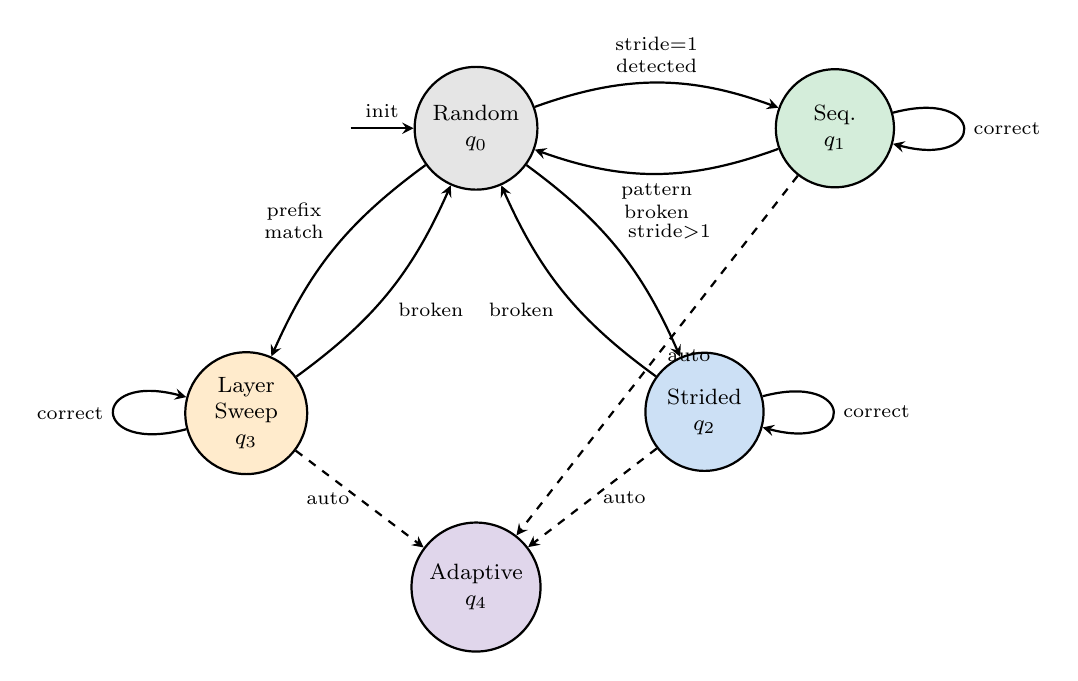
\begin{tikzpicture}[
    node distance=2cm,
    state/.style={circle, draw, thick, minimum size=1.5cm, align=center, font=\footnotesize},
    seq/.style={state, fill=solutiongreen!20},
    str/.style={state, fill=ucxblue!20},
    lsw/.style={state, fill=cudaorange!20},
    adp/.style={state, fill=neumannpurple!20},
    rnd/.style={state, fill=gray!20},
    arrow/.style={->, >=stealth, thick},
    label/.style={font=\scriptsize, align=center}
]

\node[rnd] (random) {Random\\$q_0$};
\node[seq, right=3cm of random] (seq) {Seq.\\$q_1$};
\node[str, below right=2.5cm and 1.8cm of random] (str) {Strided\\$q_2$};
\node[lsw, below left=2.5cm and 1.8cm of random] (lsw) {Layer\\Sweep\\$q_3$};
\node[adp, below=4.2cm of random] (adp) {Adaptive\\$q_4$};

\draw[arrow] ($(random.west)+(-0.8,0)$) -- (random) node[midway, above, font=\scriptsize] {init};

\draw[arrow, bend left=20] (random) to node[above, label] {stride=1\\detected} (seq);
\draw[arrow, bend left=20] (seq) to node[below, label] {pattern\\broken} (random);

\draw[arrow, bend left=15] (random) to node[above right, label] {stride$>$1} (str);
\draw[arrow, bend left=15] (str) to node[below left, label] {broken} (random);

\draw[arrow, bend right=15] (random) to node[above left, label] {prefix\\match} (lsw);
\draw[arrow, bend right=15] (lsw) to node[below right, label] {broken} (random);

\draw[arrow, dashed] (seq) to node[right, label] {auto} (adp);
\draw[arrow, dashed] (str) to node[right, label] {auto} (adp);
\draw[arrow, dashed] (lsw) to node[left, label] {auto} (adp);

\draw[arrow] (seq) to[loop right] node[label] {correct} (seq);
\draw[arrow] (str) to[loop right] node[label] {correct} (str);
\draw[arrow] (lsw) to[loop left] node[label] {correct} (lsw);

\end{tikzpicture}%
}
\caption{Prefetch engine state machine. The Adaptive strategy delegates to the detected pattern. State transitions occur when \texttt{classify\_pattern} analyzes the access history buffer (1024 entries).}
\label{fig:prefetch-fsm}
\end{figure}

\textbf{Pillar 3: Adaptive Quantization.} Hypothesis: MXFP4 quantization~\cite{rouhani2023mxfp4} achieves 4$\times$ bandwidth reduction with less than 1\% accuracy loss for inference-time KV cache transfers.

\subsection{UET-HTSIM Simulation}

Before hardware deployment, we validate the WFA classifier and adaptive routing using the Ultra Ethernet Consortium's HTSIM simulator: model the cluster topology, generate traffic matrices matching LLM patterns (incast, KV scatter, point-to-point activations), and compare Flow Completion Time distributions against baseline.

\subsection{Performance Targets}

\begin{table}[htbp]
\centering
\caption{Unified target performance metrics}
\label{tab:unified-targets}
\begin{tabular}{@{}llcc@{}}
\toprule
\textbf{Pillar} & \textbf{Metric} & \textbf{Baseline} & \textbf{Target} \\
\midrule
\multirow{2}{*}{Precision} & Stochastic round overhead & -- & $< 5\%$ \\
 & Conversion throughput & -- & $> 50$ GB/s \\
\midrule
\multirow{2}{*}{Prefetching} & Hit rate (inference) & 0\% & $> 90\%$ \\
 & Hit rate (fine-tuning) & 0\% & $> 70\%$ \\
\midrule
\multirow{2}{*}{Quantization} & $\Delta$PPL (MXFP4 KV) & FP32 & $< 0.5$ \\
 & Bandwidth reduction & 1$\times$ & 2--4$\times$ \\
\midrule
\multirow{2}{*}{System} & TTFT reduction & Current vLLM & 30--50\% \\
 & RoCE session stability & 90 s & $>$24 h \\
\bottomrule
\end{tabular}
\end{table}

\subsection{Ablation Studies}

\begin{itemize}
    \item WFA classifier vs.\ static hot/cold assignment
    \item Hot-path only vs.\ dual-path routing
    \item NUMA-aware vs.\ NUMA-oblivious allocation
    \item Threshold sensitivity analysis ($\theta_1$, $\theta_2$, $t_{\text{idle}}$)
\end{itemize}

%=============================================================================
\section{Implementation Roadmap: Project Breakdown}
\label{sec:roadmap}
%=============================================================================

The thesis implementation is organized as independent, self-contained projects. Each project has clear inputs, outputs, and success criteria, enabling parallel development and incremental validation.

\subsection{Completed Projects}

\begin{table}[htbp]
\centering
\caption{Completed thesis projects with deliverables}
\label{tab:completed-projects}
\small
\resizebox{\textwidth}{!}{%
\begin{tabular}{@{}clll@{}}
\toprule
\textbf{\#} & \textbf{Project} & \textbf{Deliverables} & \textbf{Section} \\
\midrule
P1 & Cluster Deployment & Phase 1 lab cluster (Chimera/Cerberus/Hydra), Soft-RoCE baseline (0.92~Gb/s, 189~$\mu$s) & \S\ref{sec:hardware}, \S\ref{sec:softroce-baseline} \\
P2 & FlashAttention 3 Fix & Lazy import patch for vLLM Blackwell support, +15.5\% vLLM throughput on RTX 5090 & \S\ref{sec:fa3-fix} \\
P3 & TCP Benchmarks & gpt-oss-120b baseline (104.42~tok/s), single-node vs multi-node analysis & \S\ref{sec:benchmarks} \\
P4 & Transport Middleware & TransportBase abstraction, TCP/RoCE/TTPoe implementations, TransportSelector, NCCLConfig & \S\ref{sec:architecture} \\
P5 & EXO Integration & RDMADiscovery, RDMATransport, RDMATopologyManager (639 lines) & \S\ref{sec:architecture} \\
P6 & Critical Issues Analysis & 7 blocking issues across NCCL/UCX/vLLM with proposed solutions & \S\ref{sec:critical-issues} \\
P7 & System Architecture & WFA classifier, dual-path routing, RDMA Tensor Cache design & \S\ref{sec:architecture} \\
P8 & Neumann Crate & \texttt{tensor\_rdma} Rust crate (116 tests, clean): precision, rounding, prefetch, transport, cache, config & \S\ref{sec:rdma-cache} \\
\bottomrule
\end{tabular}%
}
\end{table}

\subsection{Remaining Projects}

\begin{table}[htbp]
\centering
\caption{Remaining thesis projects with success criteria}
\label{tab:remaining-projects}
\small
\resizebox{\textwidth}{!}{%
\begin{tabular}{@{}clll@{}}
\toprule
\textbf{\#} & \textbf{Project} & \textbf{Deliverables} & \textbf{Success Criteria} \\
\midrule
P9 & Hardware RoCE & ConnectX-4 firmware, \texttt{ib\_write\_bw}/\texttt{ib\_write\_lat}, GPUDirect on V100 & Latency $<$5~$\mu$s, BW $>$80~Gb/s \\
P10 & WFA Integration & Classifier in vLLM connector, telemetry, phase detection & $>$90\% accuracy on synthetic patterns \\
P11 & Precision Pipeline & End-to-end FP16$\to$FP32$\to$BF16, Tower 1$\leftrightarrow$Tower 2 & $<$5\% overhead, unbiased gradients \\
P12 & Prefetch Engine & Adaptive FSM + RDMA cache, pattern detection & $>$90\% hit (inference), $>$70\% (fine-tune) \\
P13 & MXFP4 Quantization & KV cache quantization for bandwidth reduction & 4$\times$ reduction, $<$1\% PPL loss \\
P14 & UET-HTSIM Simulation & WFA + routing validated in UEC simulator & FCT improvement over baseline \\
P15 & End-to-End Eval & Full pipeline: TTFT, throughput, ablation studies & 30--50\% TTFT, $>$24h RoCE stability \\
P16 & Thesis Writing & Consolidated report with all experimental results & Defense-ready document \\
\bottomrule
\end{tabular}%
}
\end{table}

\subsection{Project Dependencies}

Projects P9--P11 can proceed in parallel. P12 depends on P8 (Neumann crate). P13--P14 can proceed independently. P15 requires P9--P13. P16 runs continuously alongside all projects.

%=============================================================================
\section{Future Work and Conclusions}
\label{sec:conclusions}
%=============================================================================

\subsection{UCX/UCC Integration Path}

The middleware's transport abstraction maps directly to UCX transport layers. A recent RFC for vLLM~\cite{vllm-ucc-rfc} proposes replacing NCCL with UCC for environments where NCCL's CUDA dependency is a limitation. For our cluster, UCX transport negotiation would handle the heterogeneous path (TCP for Tower~1, RoCE for Tower~2) automatically via \texttt{UCX\_TLS=rc,tcp}.

UEC~1.0~\cite{uec2025} defines native multipath with packet spraying, ordered delivery without HOL blocking, built-in congestion control for incast, and selective retransmission---all designed for AI/HPC workloads. The middleware's transport abstraction is designed to accommodate UEC as an additional backend when available.

\subsection{RISC-V Assembly Generation}

A secondary research direction involves fine-tuning an LLM to generate RISC-V assembly code, leveraging the distributed infrastructure and adaptive RDMA middleware developed in this thesis for gradient synchronization during training.

\subsection{Conclusions}

This report consolidates the research progress from Updates 2--11, presenting a unified view of the adaptive RDMA optimization framework for distributed LLM workloads. The key contributions are:

\begin{enumerate}
    \item \textbf{Comprehensive issue analysis}: Seven critical blocking issues identified across NCCL, UCX, and vLLM, with proposed solutions for each.
    \item \textbf{Adaptive middleware}: A WFA-based tensor classifier with dual-path routing that differentiates latency-sensitive from throughput-sensitive transfers.
    \item \textbf{RDMA Tensor Cache}: A precision management layer in Neumann that resolves heterogeneous GPU precision mismatches through FP32 master weight storage and stochastic rounding.
    \item \textbf{Pluggable transport}: Support for TCP, Soft-RoCE, hardware RoCE, and TTPoe through a unified abstraction, with integration into both vLLM and exo frameworks.
    \item \textbf{Experimental validation framework}: Three-pillar methodology targeting precision overhead, prefetch effectiveness, and quantization quality, with concrete performance targets.
    \item \textbf{Circuit-aware transport}: Analysis of Anthropic's Transformer Circuits research identifies five concrete gaps in the middleware and proposes circuit-aware enhancements---composition-weighted WFA, phase-aware precision, sparse RDMA transfers, head-type prefetching, and delta-mode pipeline transport---with estimated 40--200$\times$ bandwidth compression on sparse-activation workloads.
\end{enumerate}

The work demonstrates that intelligent communication scheduling---treating tensor transfers as first-class objects with metadata-driven routing---can achieve latency improvements on consumer hardware that previously required expensive InfiniBand deployments.

%=============================================================================
% Back Matter
%=============================================================================

\bibliographystyle{plainnat}
\bibliography{update10}

\appendix

\section{Scripts and Configurations}
\label{app:scripts}

All implementation code, deployment configurations, and benchmark scripts are provided in the \texttt{scripts/} directory alongside this document:

\begin{table}[htbp]
\centering
\small
\resizebox{\textwidth}{!}{%
\begin{tabular}{@{}lll@{}}
\toprule
\textbf{File} & \textbf{Type} & \textbf{Purpose} \\
\midrule
\texttt{wfa\_classifier.py} & Python & WFA tensor classifier and phase detection \\
\texttt{dual\_path\_rdma.py} & Python & Hot/cold QP pool routing \\
\texttt{rdma\_buffer\_pool.py} & Python & NUMA-aware pyverbs buffer pool \\
\texttt{transports.py} & Python & TransportBase, TCP/RoCE/TTPoe, Selector, NCCLConfig \\
\texttt{exo\_rdma\_integration.py} & Python & RDMADiscovery, RDMATransport, TopologyManager \\
\texttt{vllm\_connector.py} & Python & AdaptiveRDMAConnector, InstrumentedKVCacheManager \\
\texttt{benchmark\_vllm.py} & Python & gpt-oss-120b inference benchmark \\
\texttt{benchmark\_transports.py} & Python & Multi-transport comparison with LaTeX output \\
\texttt{benchmark\_all.sh} & Bash & Automated benchmark across all transports \\
\texttt{start\_cluster.sh} & Bash & Unified cluster start with transport selection \\
\texttt{load\_ttpoe.sh} & Bash & TTPoe kernel module loader \\
\texttt{docker-compose.head.yaml} & YAML & Ray head node + vLLM server deployment \\
\texttt{docker-compose.worker.yaml} & YAML & Ray worker node deployment \\
\bottomrule
\end{tabular}%
}
\caption{Scripts and configuration files provided with this report}
\end{table}

\section{Expected Transport Performance}
\label{app:transport-performance}

Based on prior testing (Section~\ref{sec:softroce-baseline}) and transport specifications:

\begin{table}[htbp]
\centering
\small
\begin{tabular}{@{}lcccc@{}}
\toprule
\textbf{Transport} & \textbf{Latency} & \textbf{Expected Throughput} & \textbf{CPU Overhead} & \textbf{Status} \\
\midrule
TCP & $\sim$1 ms & Baseline & High & Always available \\
Soft-RoCE & $\sim$190 $\mu$s & +10--15\% & Medium & Deprecated \\
Hardware RoCE & $<$2 $\mu$s & +15--25\% & Low & Requires Mellanox \\
Tesla TTPoe & $\sim$2 $\mu$s & +20--30\% & Near-zero & Requires module \\
\bottomrule
\end{tabular}
\caption{Expected transport performance for distributed LLM inference}
\end{table}

\begin{figure}[htbp]
\centering
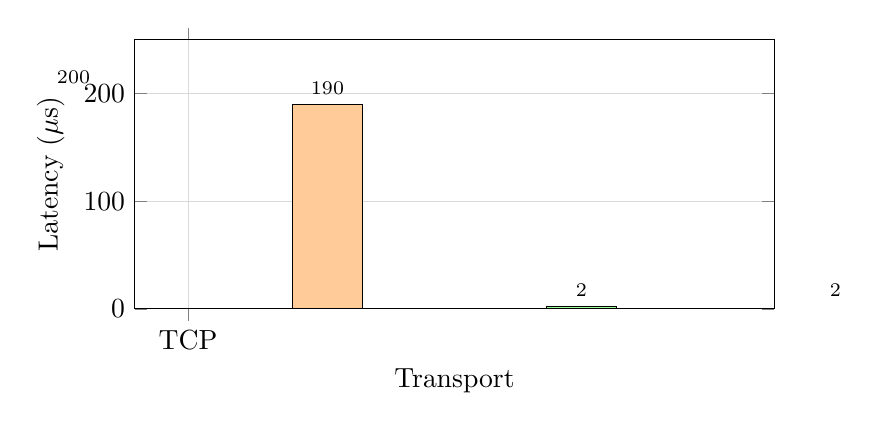
\begin{tikzpicture}
\begin{axis}[
    ybar,
    bar width=0.9cm,
    width=0.8\textwidth,
    height=5cm,
    ylabel={Latency ($\mu$s)},
    xlabel={Transport},
    ymin=0,
    ymax=250,
    symbolic x coords={TCP, Soft-RoCE, Hardware RoCE, TTPoe},
    xtick=data,
    nodes near coords,
    every node near coord/.append style={font=\scriptsize},
    grid=major,
    grid style={gray!30},
]
\addplot[fill=gray!40] coordinates {(TCP, 200)};
\addplot[fill=orange!40] coordinates {(Soft-RoCE, 190)};
\addplot[fill=green!40] coordinates {(Hardware RoCE, 2)};
\addplot[fill=purple!40] coordinates {(TTPoe, 2)};
\end{axis}
\end{tikzpicture}
\caption{Transport latency comparison---TCP baseline vs RDMA alternatives. Hardware RoCE and TTPoe achieve 100$\times$ lower latency than software solutions.}
\label{fig:transport-latency-comparison}
\end{figure}

\end{document}
